\chapter{bijlagen}

\section{test2: Dataoverdracht in subview's}
\paragraph{View ververs aantal en ververs tijd }
%viewrefreshtime
% Binding test 1
\subsection{Binding}
\begin{figure}[H]
    \centering
    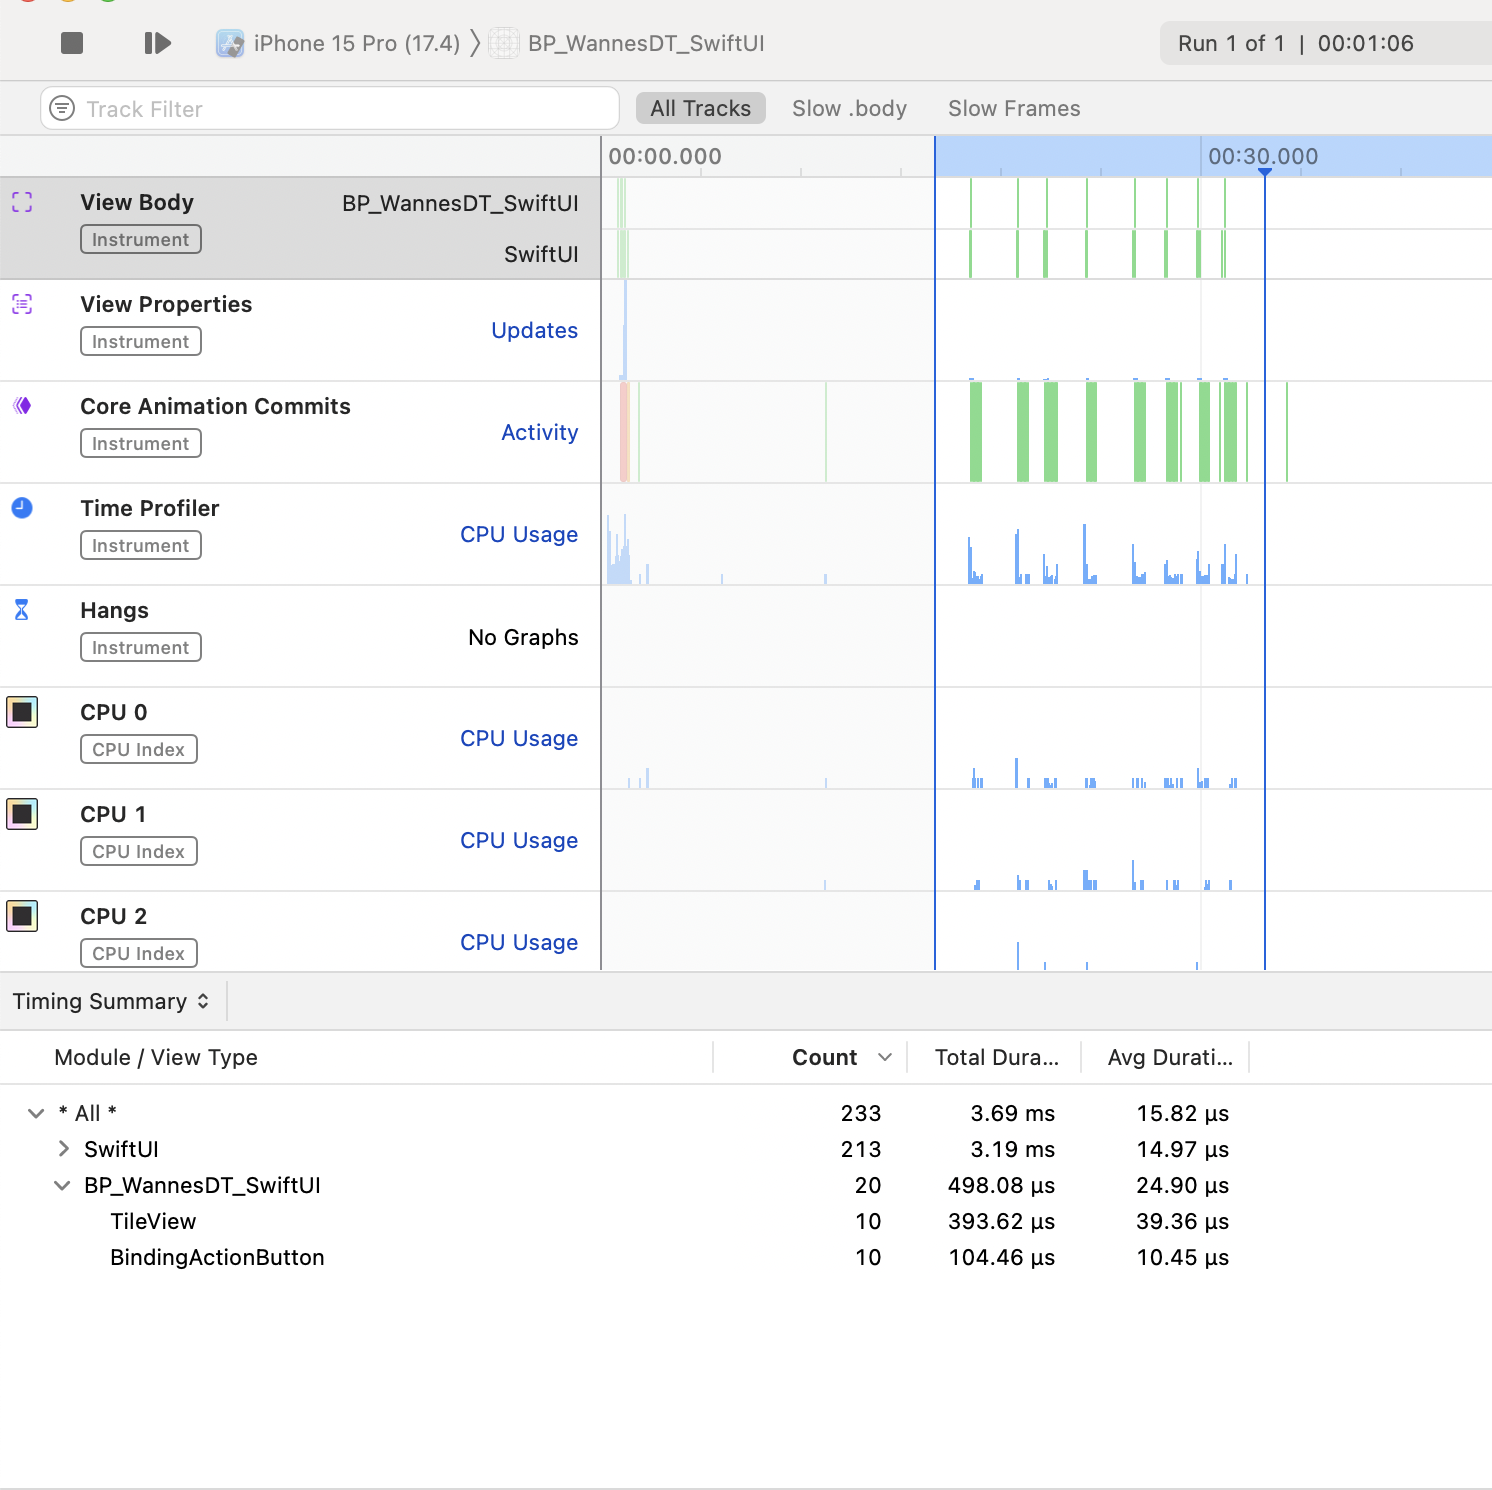
\includegraphics[width=0.7\textwidth]{bptest1_insubview/BindingButtonPressViewRefreshesAndTime} 
    \caption{test2: Aantal keren dat de view refreshed en gemiddelde duratie bij het meervoudig toewijzigen van een binding}
    \label{fig:viewRefreshesBinding1}
\end{figure}
\paragraph{Aantal updates van property's}
\begin{figure}[H]
    \centering
    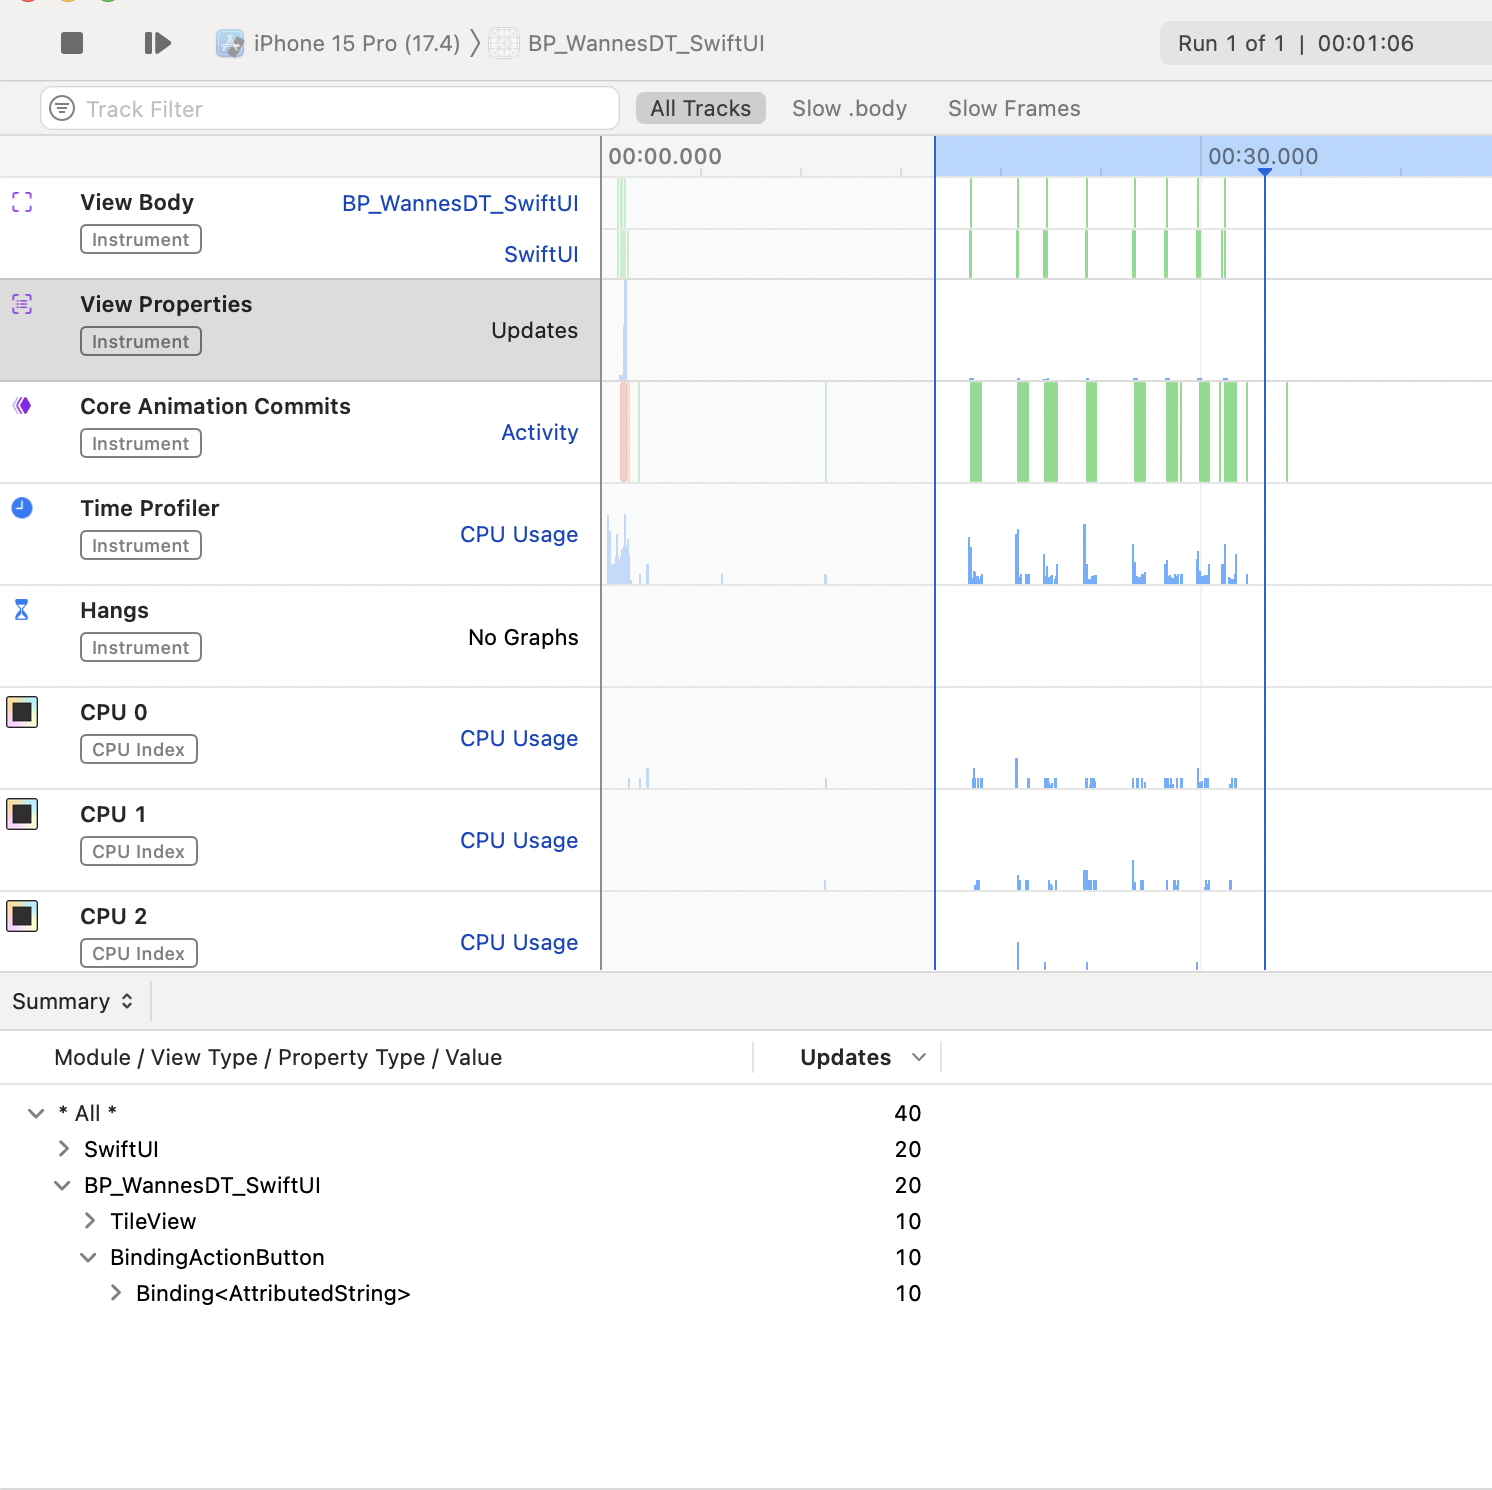
\includegraphics[width=0.7\textwidth]{bptest1_insubview/BindingButtonPressViewPropertyUpdates} 
    \caption{test2: Aantal keren dat de property's updaten bij het meervoudig toewijzigen van een binding}
    \label{fig:propertyUpdatesBinding1}
\end{figure}
\paragraph{Totale tijd gebruikt van de CPU}
\begin{figure}[H]
    \centering
    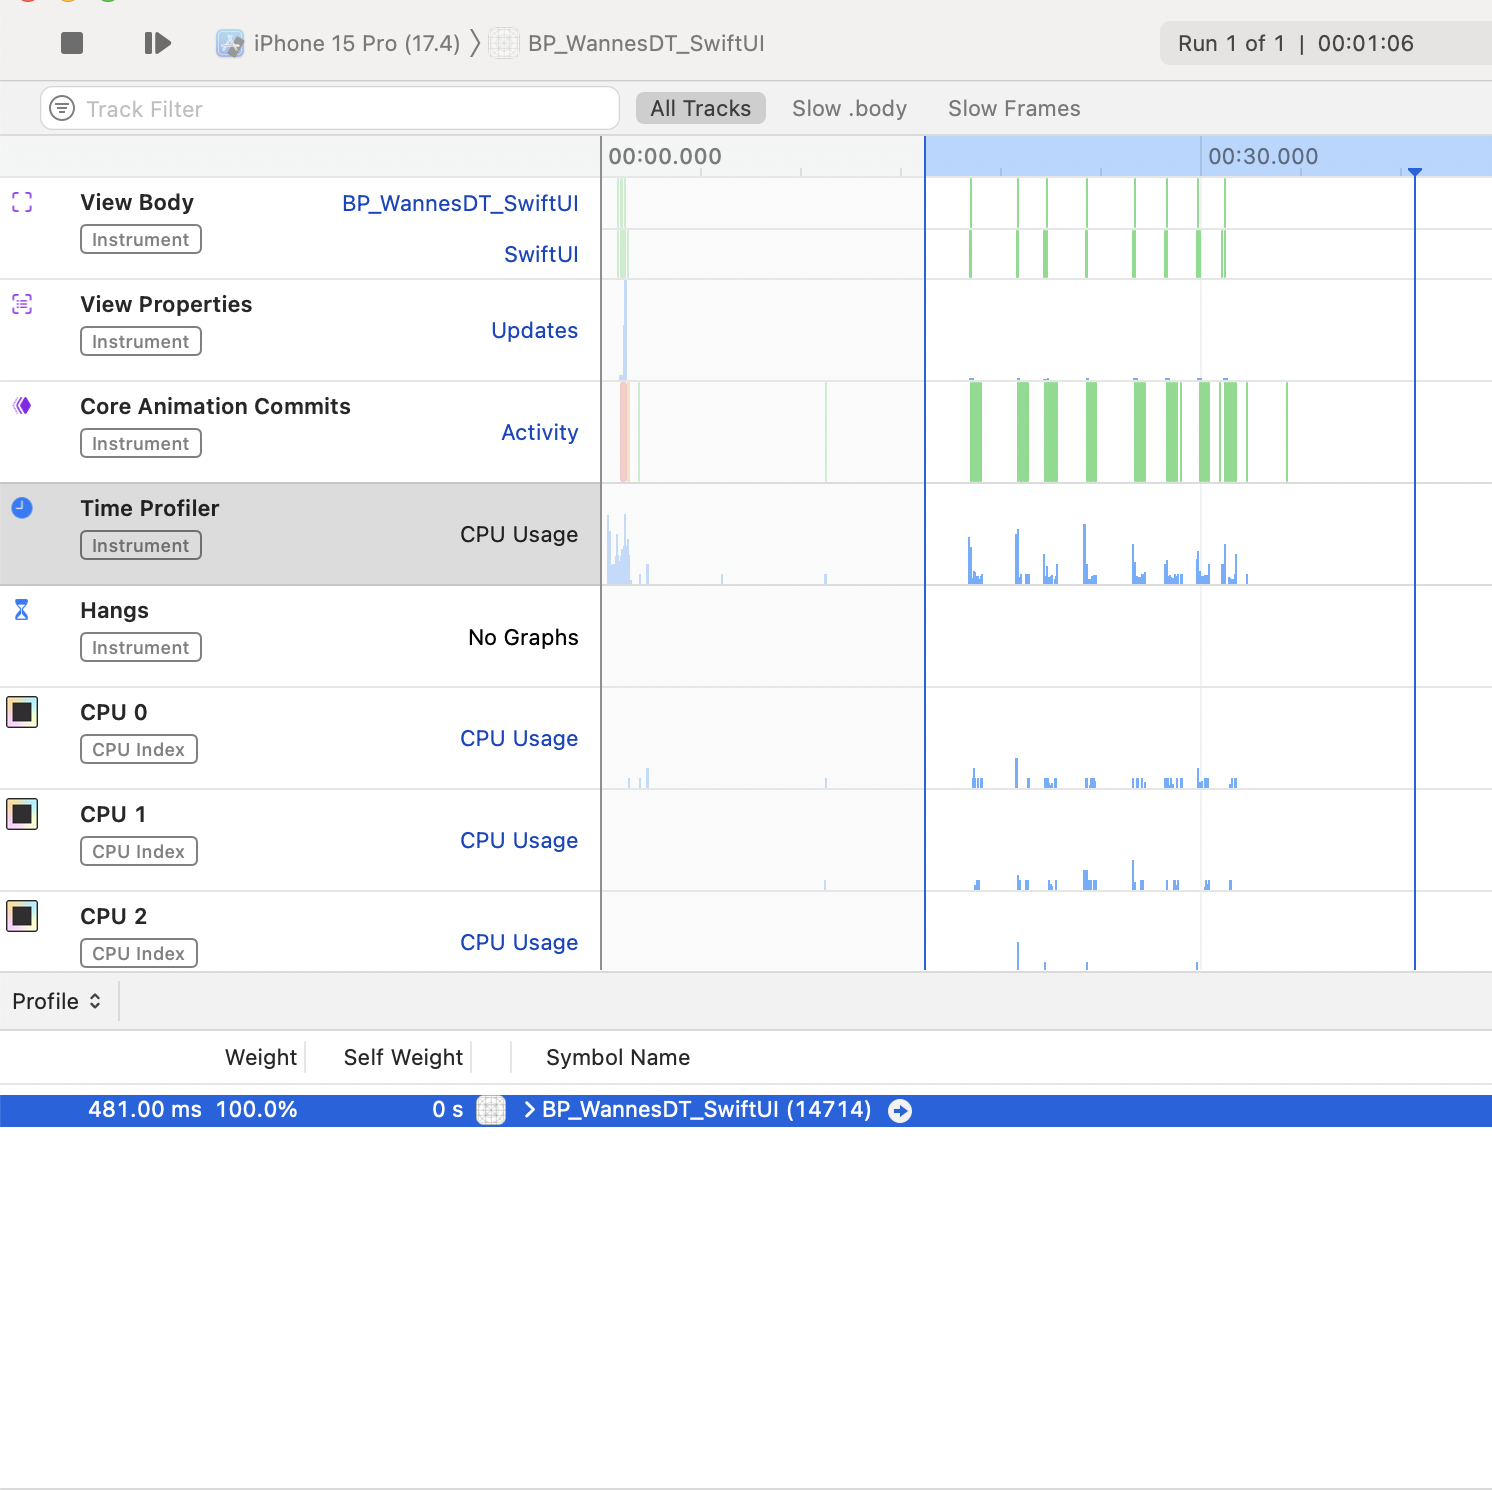
\includegraphics[width=0.7\textwidth]{bptest1_insubview/BindingButtonPressTotalCpuTime} 
    \caption{test2: De totale duratie die gebruikt is van de CPU bij het gebruik van bindings}
    \label{fig:cpuUsageTimeBinding1}
\end{figure}
\paragraph{Last op de CPU}
\begin{figure}[H]
    \centering
    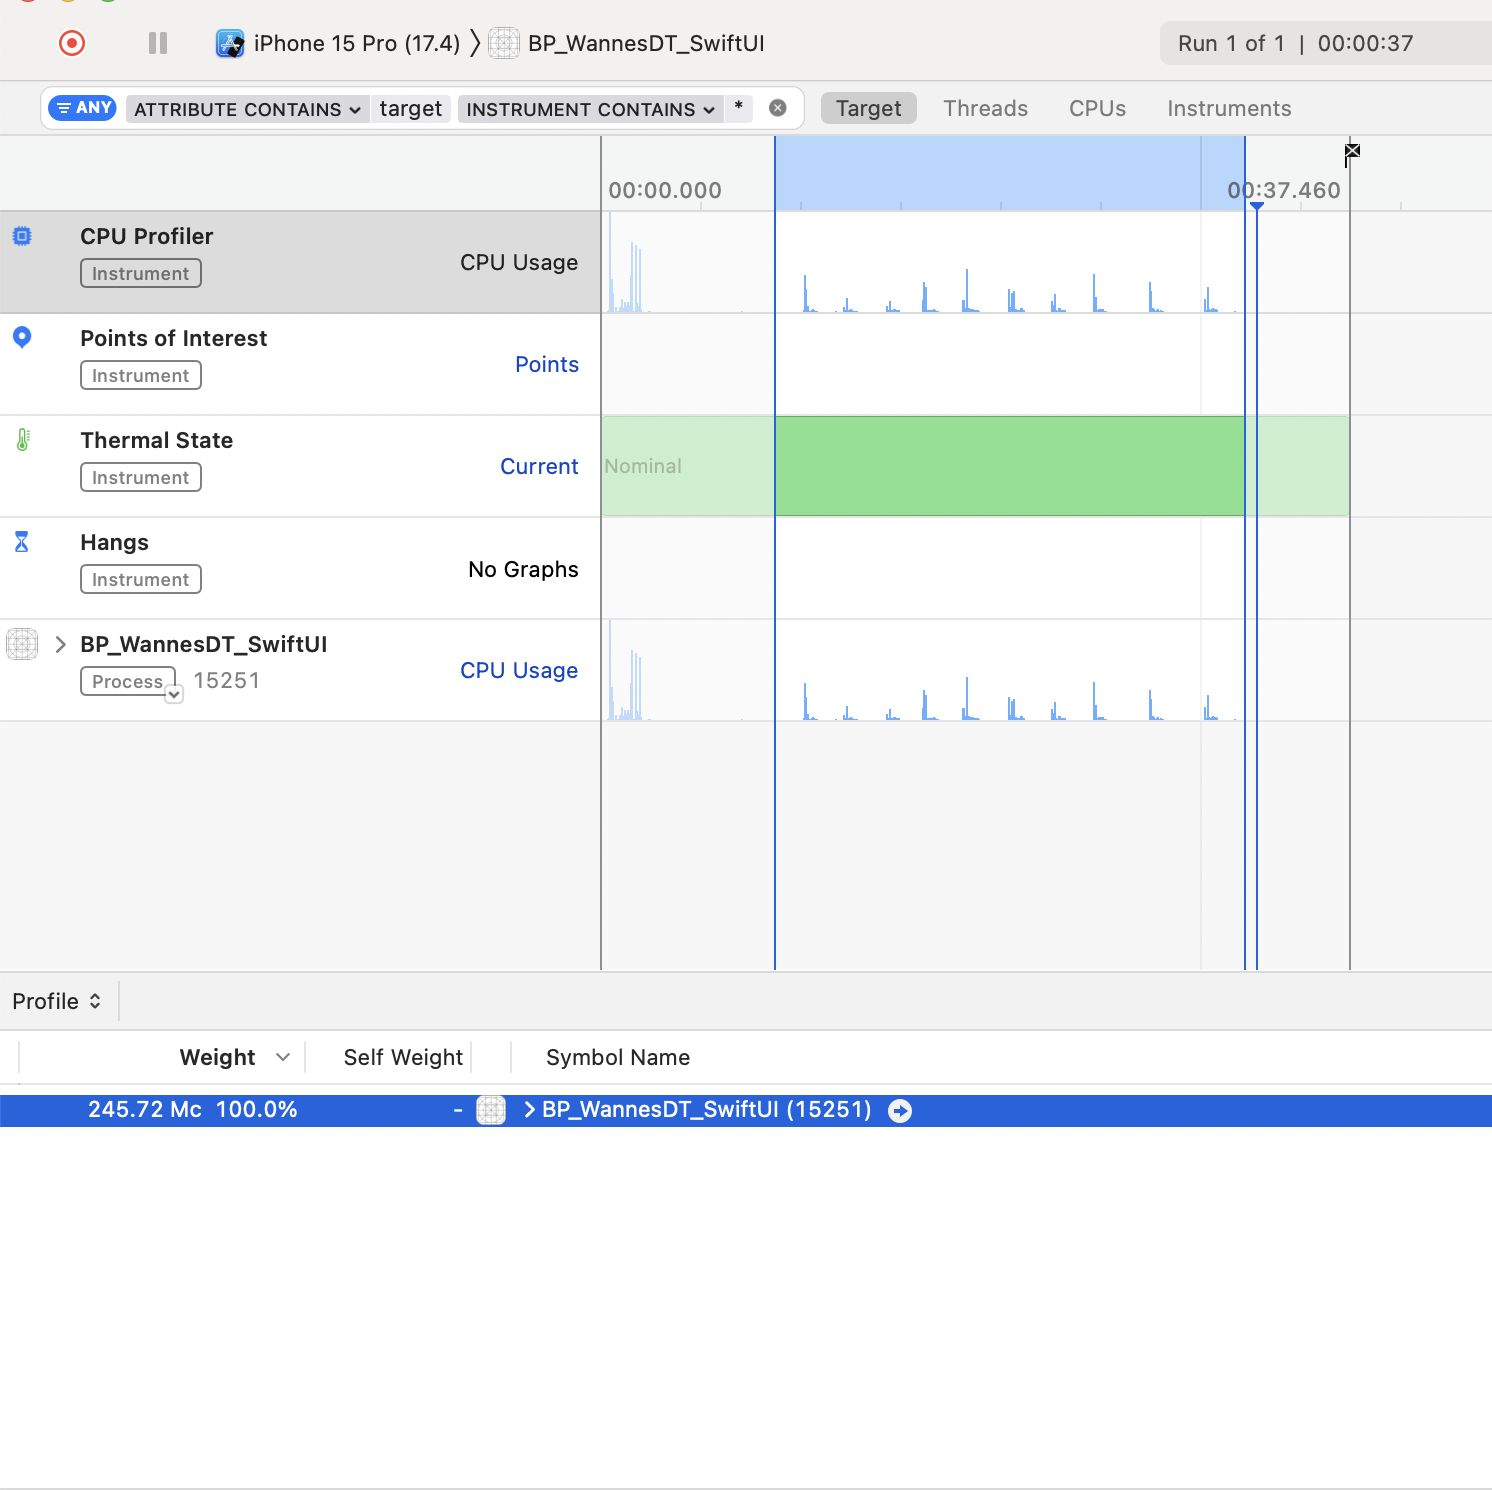
\includegraphics[width=0.7\textwidth]{bptest1_insubview/BindingButtonPressCpuUsage} 
    \caption{test2: De totale last van het opnieuw toewijzen van property's op de cpu bij het gebruik van bindings}
    \label{fig:cpuWeightBinding1}
\end{figure}

% Observable test 1
\subsection{Observable}
\paragraph{View ververs aantal en ververs tijd}
\begin{figure}[H]
    \centering
    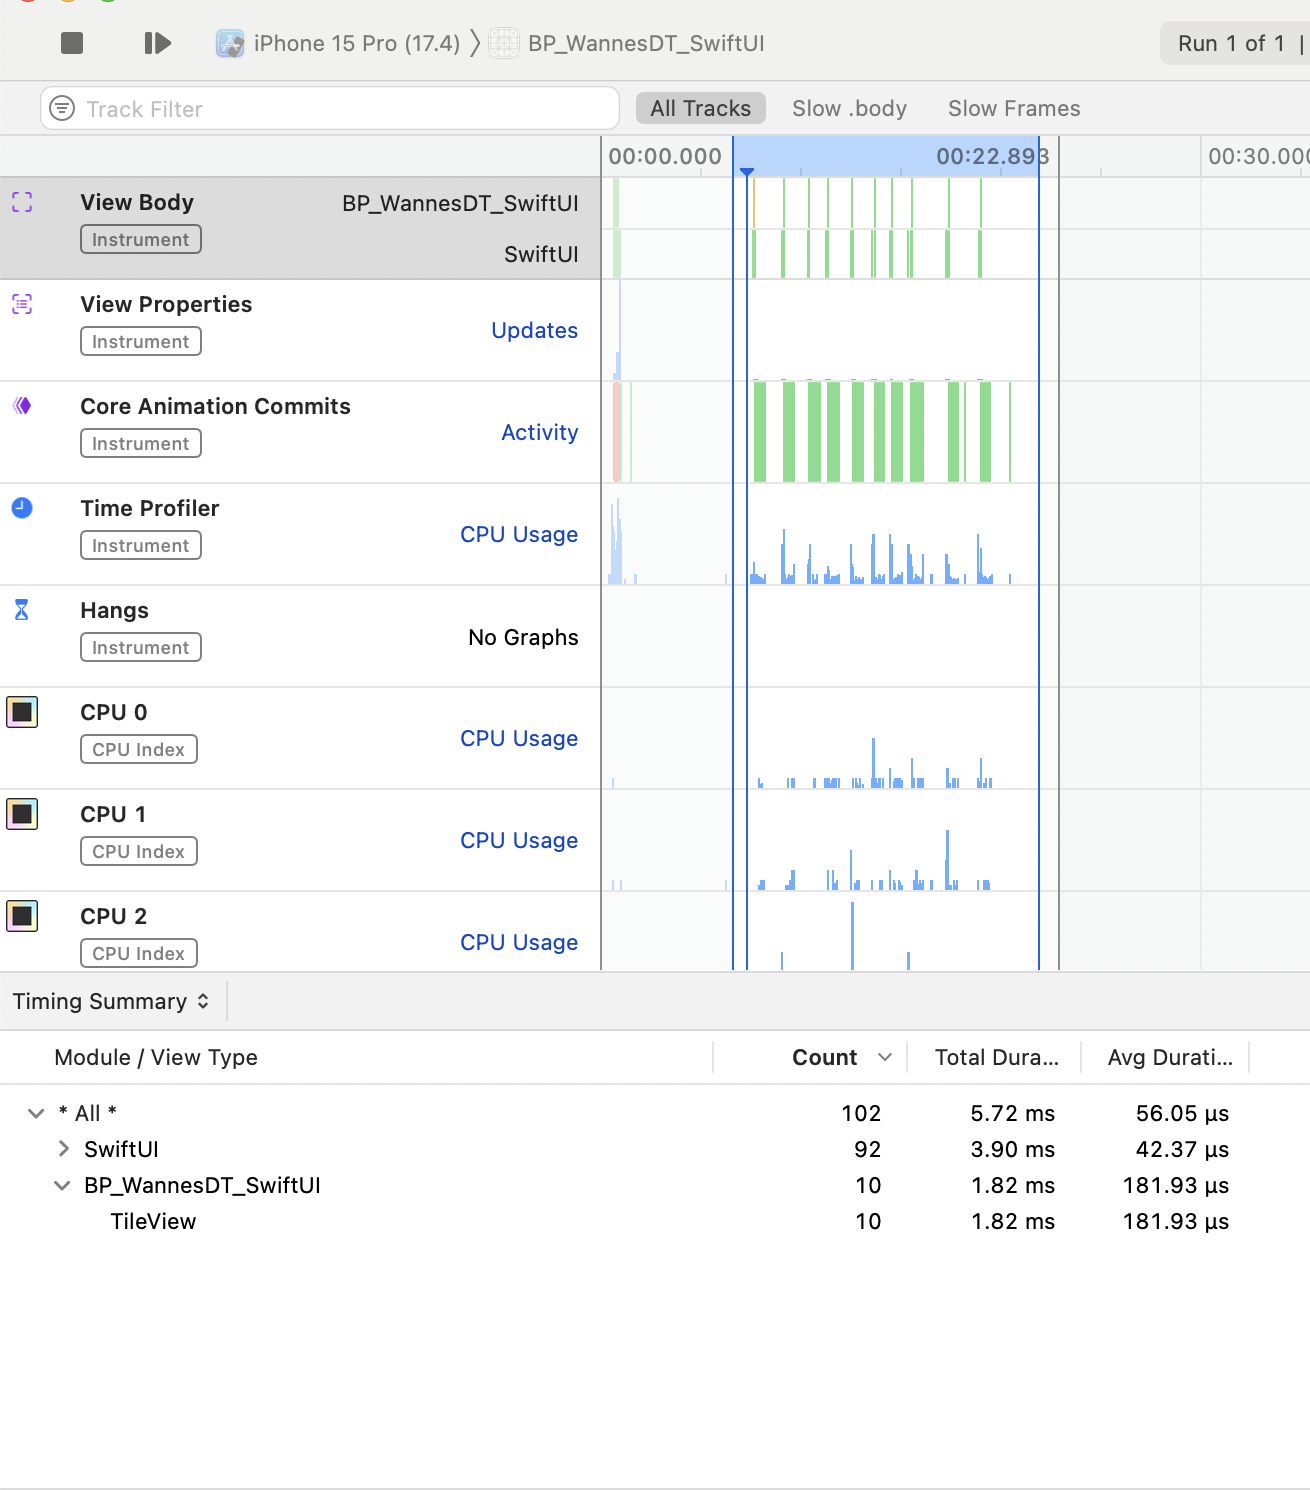
\includegraphics[width=0.7\textwidth]{bptest1_insubview/ObservableButtonPressViewRefreshesAndTime} 
    \caption{test2: Aantal keren dat de view refreshed en gemiddelde duratie bij het meervoudig toewijzigen van een Observable}
    \label{fig:viewRefreshesObservable1}
\end{figure}
\paragraph{Aantal updates van property's}
\begin{figure}[H]
    \centering
    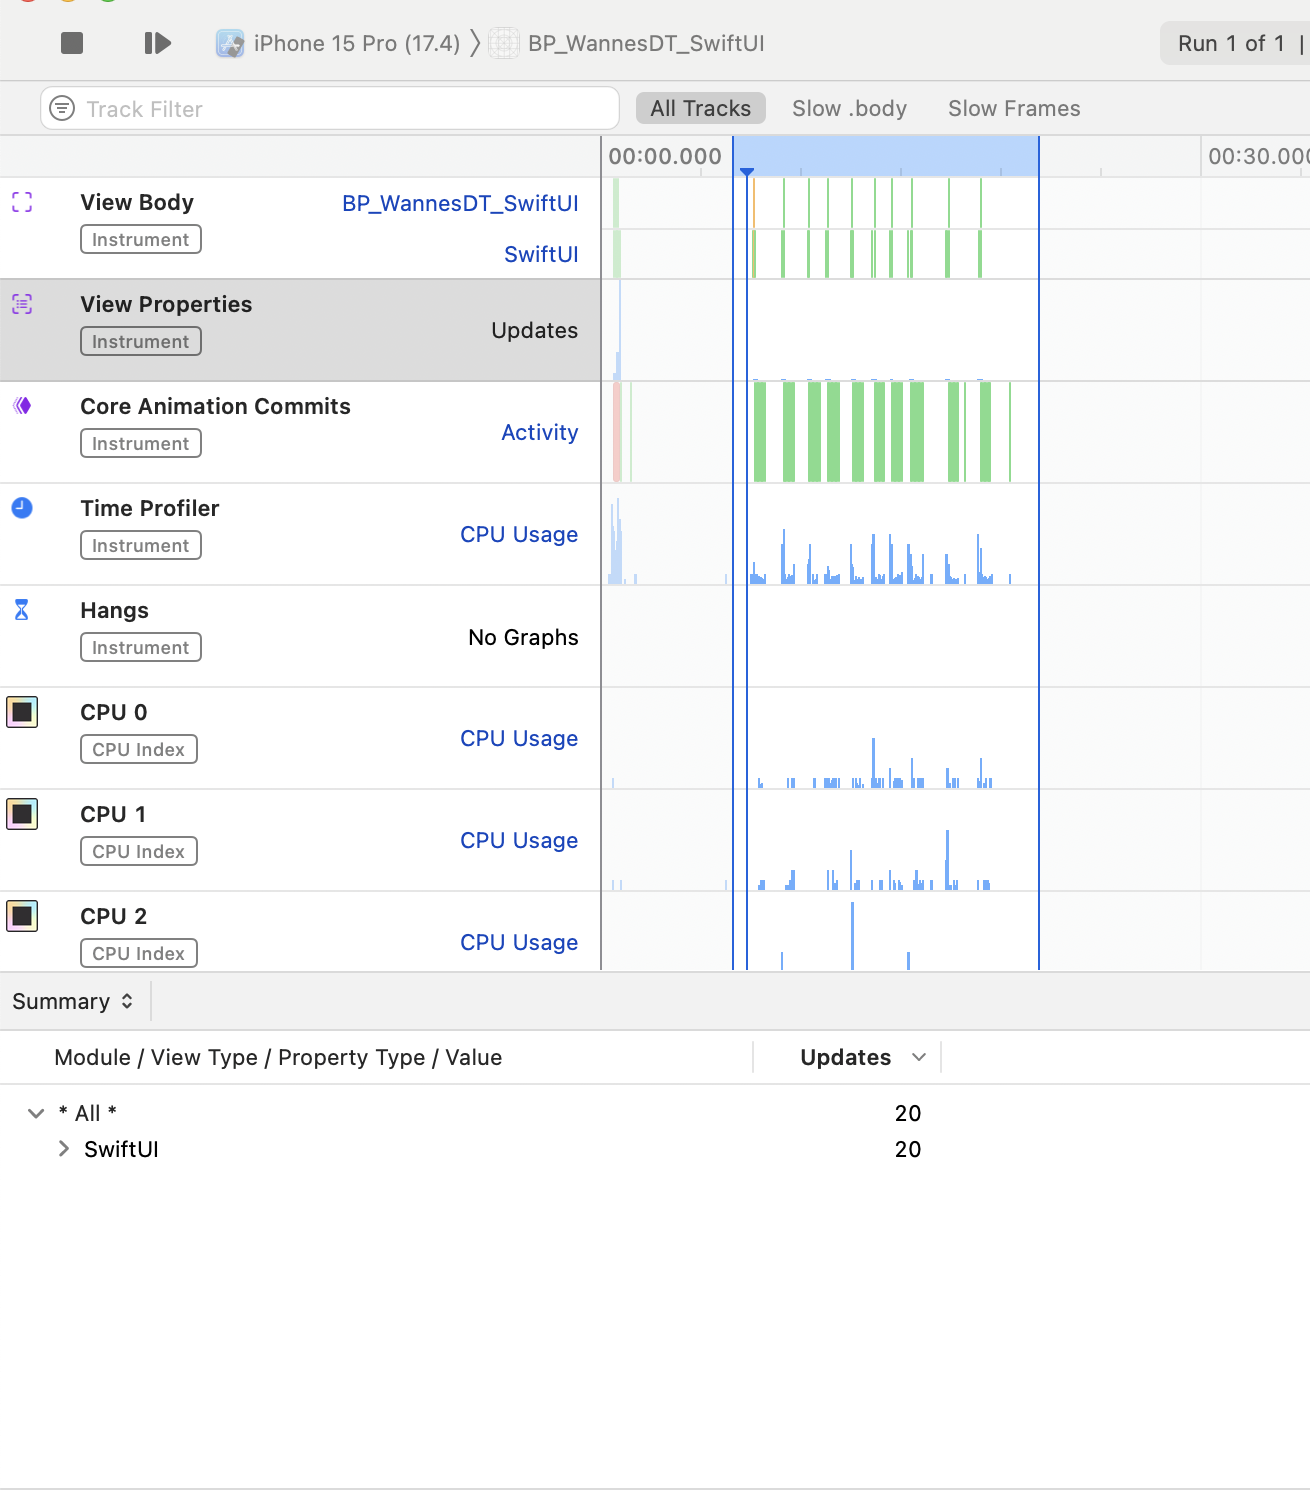
\includegraphics[width=0.7\textwidth]{bptest1_insubview/ObservableButtonPressViewPropertyUpdates} 
    \caption{test2: Aantal keren dat de property's updaten bij het meervoudig toewijzigen van een Observable}
    \label{fig:propertyUpdatesObservable1}
\end{figure}
\paragraph{Totale tijd gebruikt van de CPU}
\begin{figure}[H]
    \centering
    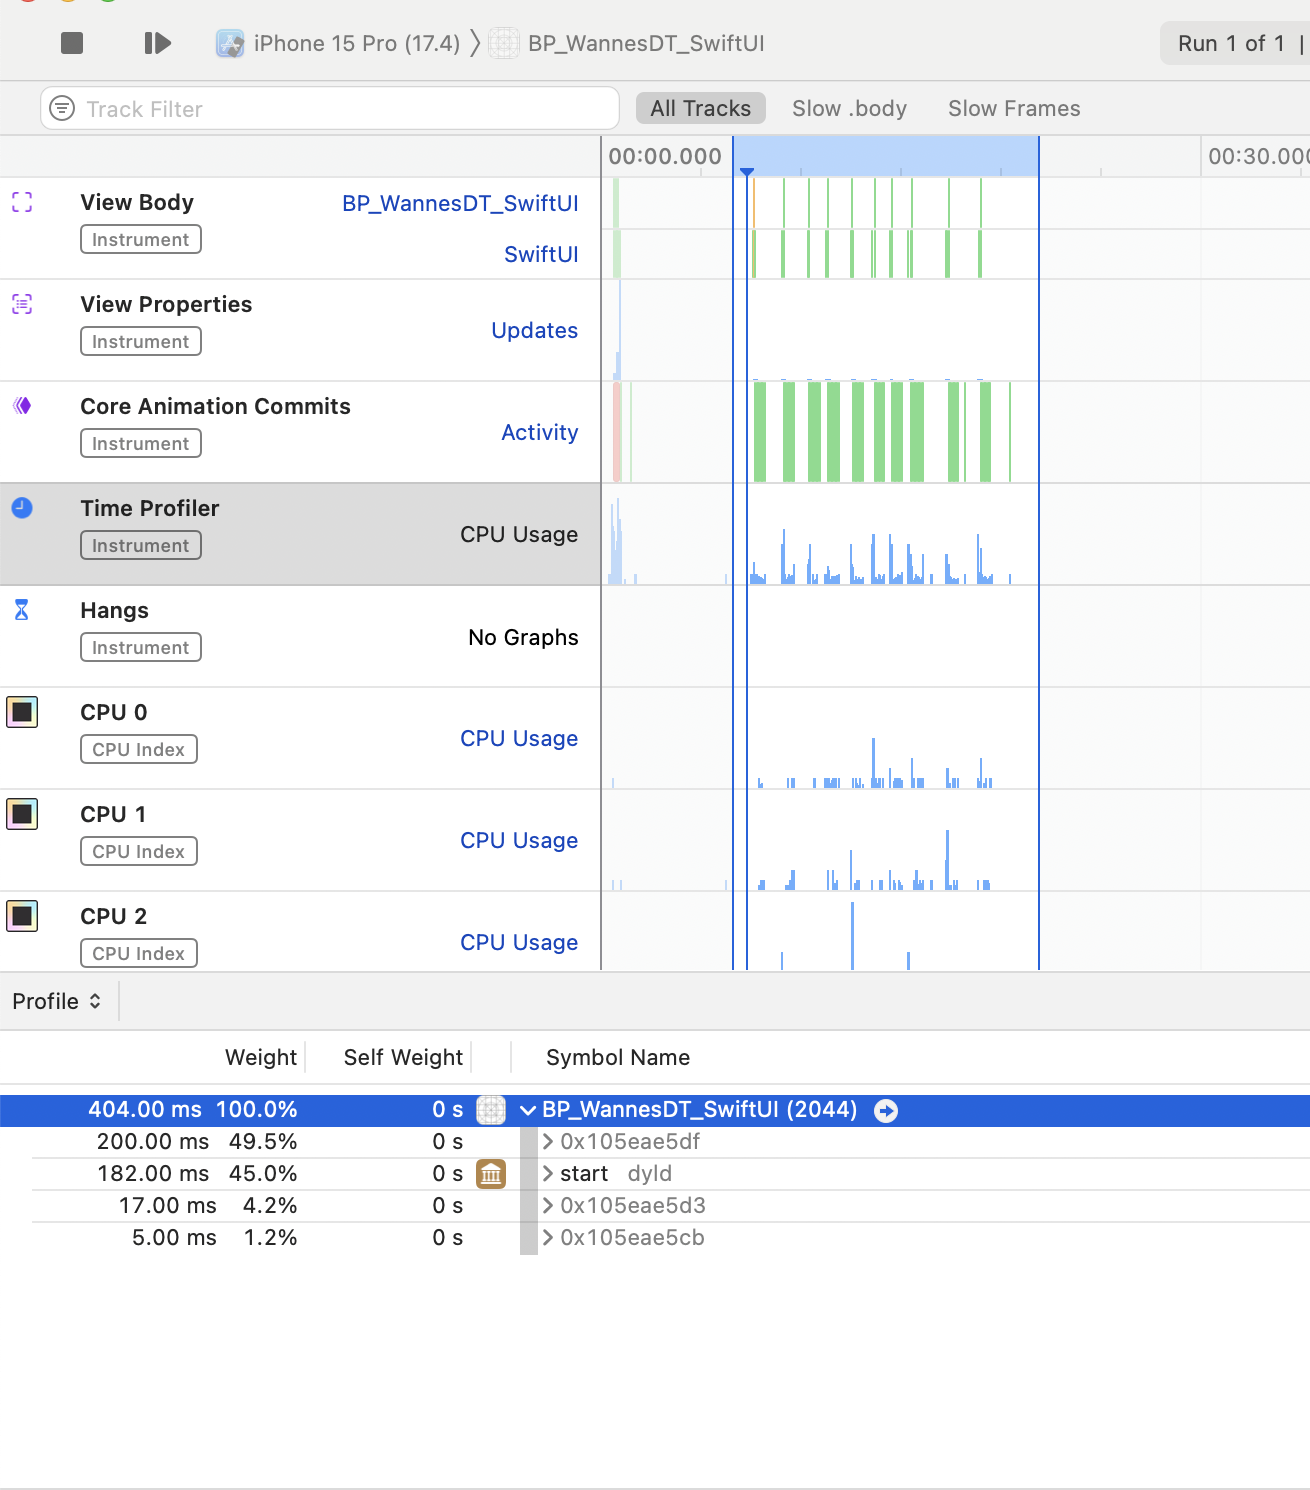
\includegraphics[width=0.7\textwidth]{bptest1_insubview/ObservableButtonPressTotalCpuTime} 
    \caption{test2: De totale duratie die gebruikt is van de CPUbij het gebruik van Observable}
    \label{fig:cpuUsageTimeObservable1}
\end{figure}
\paragraph{Last op de CPU}
\begin{figure}[H]
    \centering
    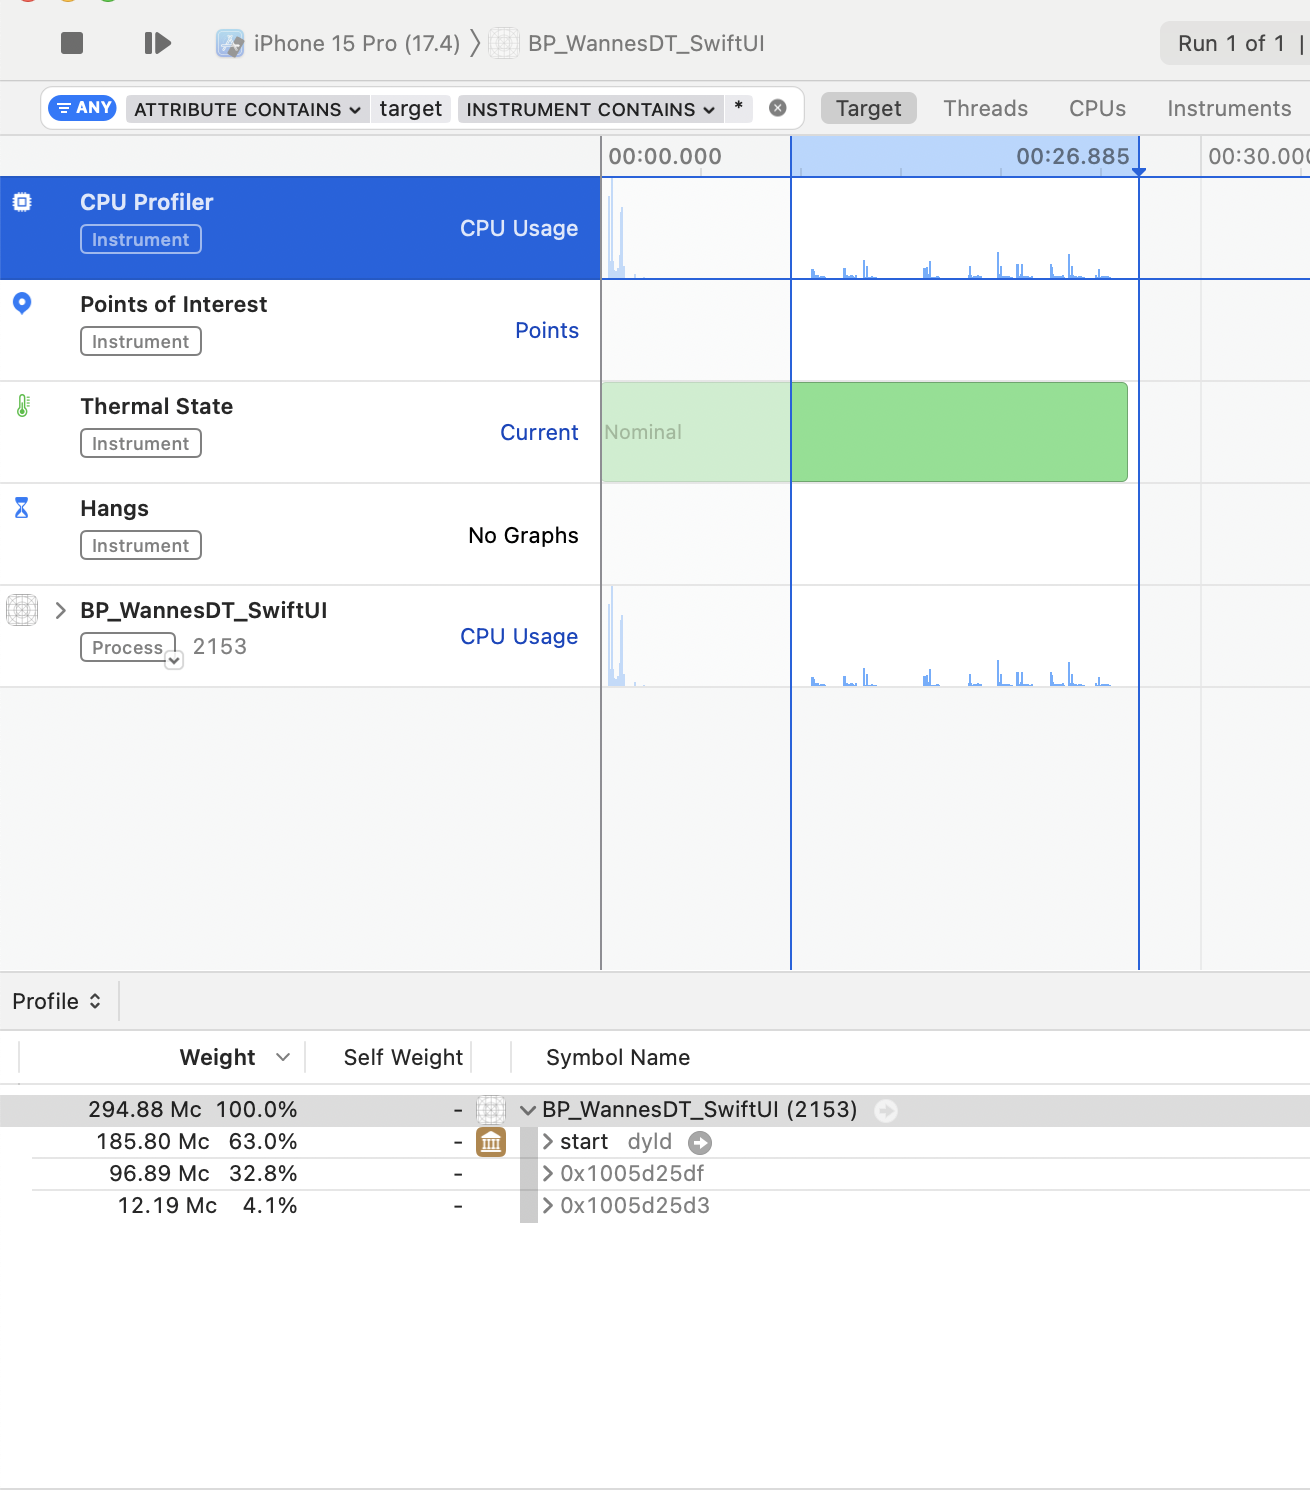
\includegraphics[width=0.7\textwidth]{bptest1_insubview/ObsrvableButtonPressCpuUsage} 
    \caption{test2: De totale last van het opnieuw toewijzen van property's op de cpu bij het gebruik van Observable}
    \label{fig:cpuWeightObservable1}
\end{figure}

\subsection{ObservedObject}
% ObservedObject test 1
\paragraph{View ververs aantal en ververs tijd}
\begin{figure}[H]
    \centering
    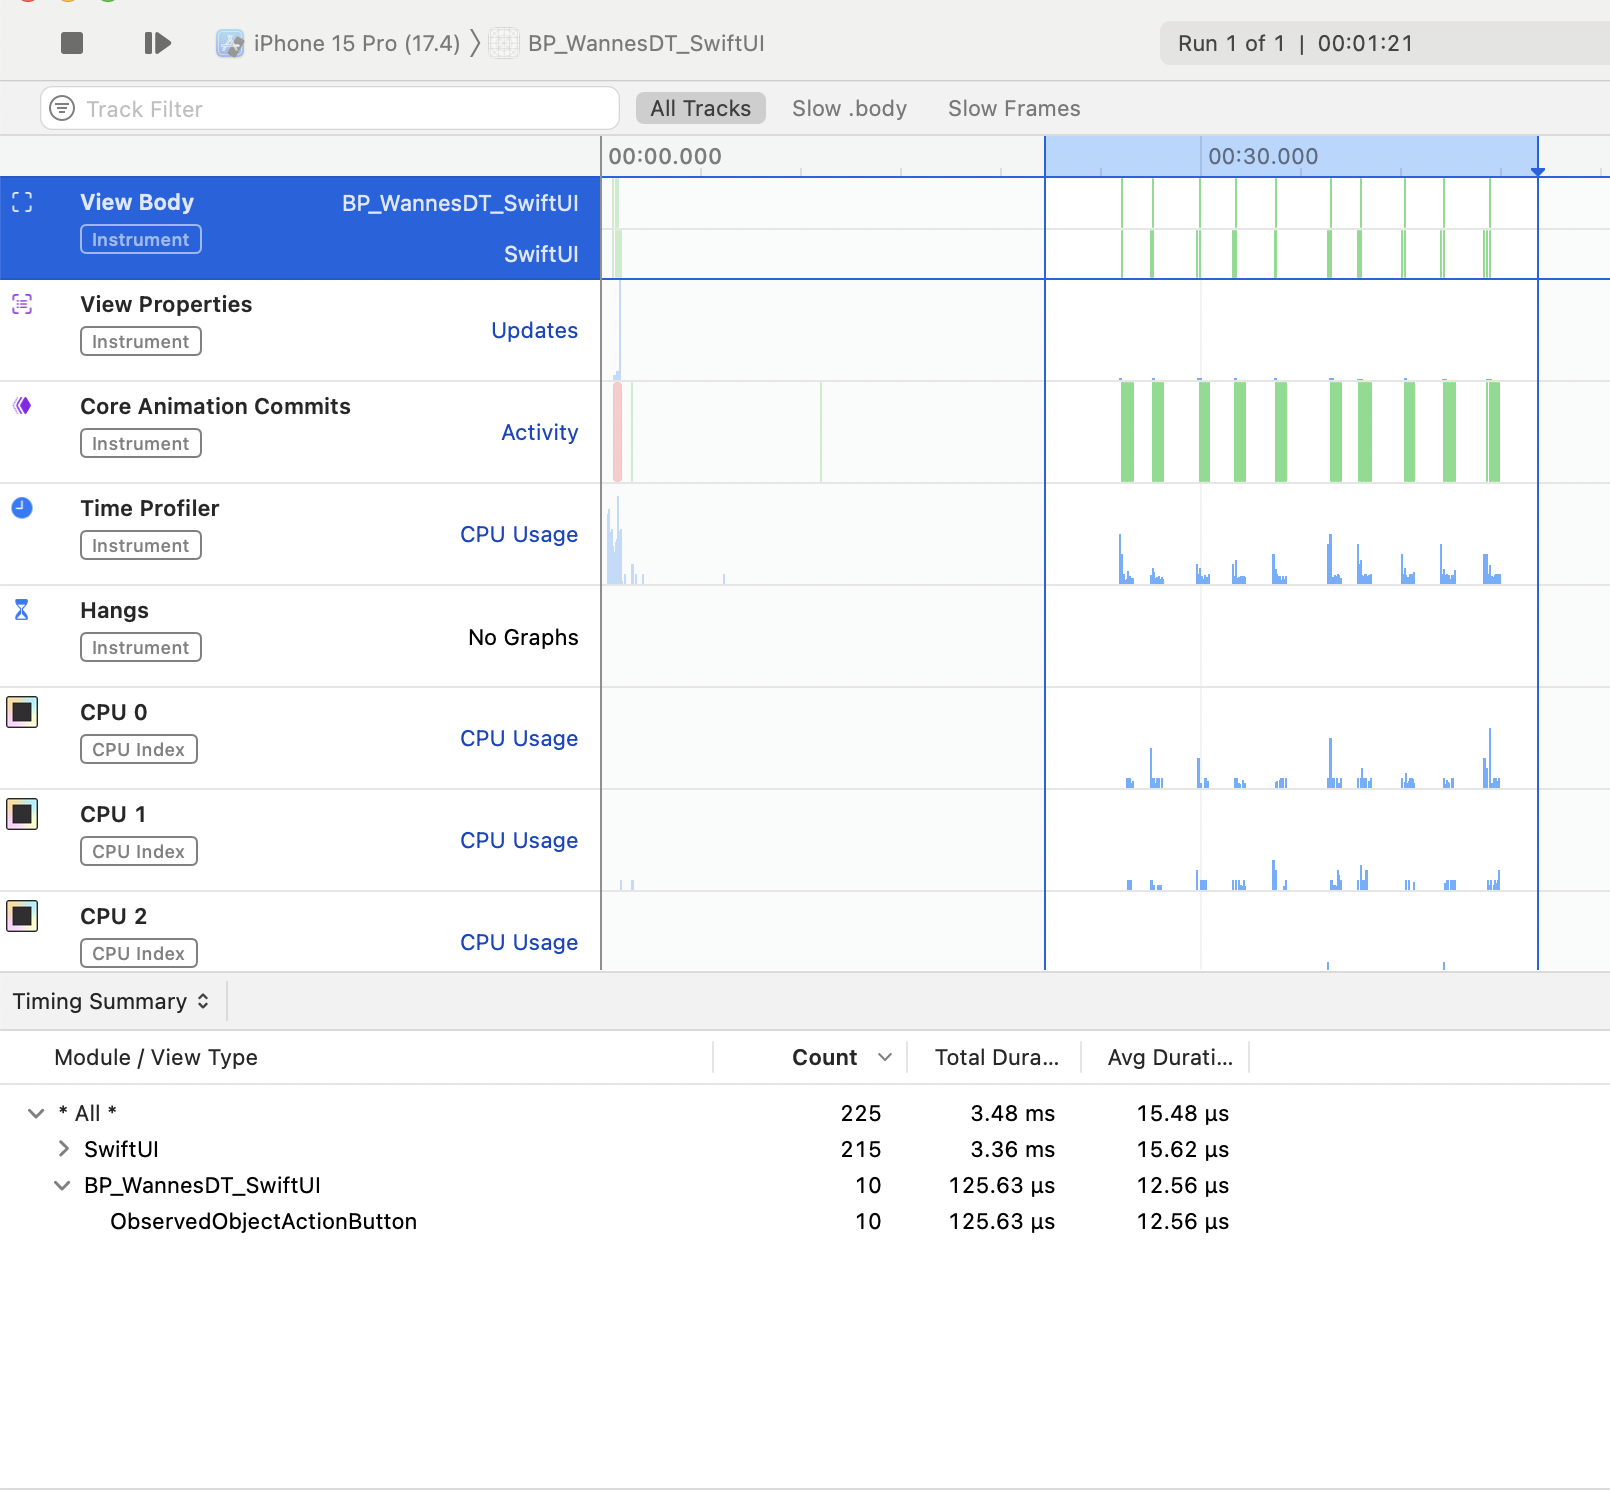
\includegraphics[width=0.7\textwidth]{bptest1_insubview/ObservableObjectButtonPressViewRefreshesAndTime} 
    \caption{test2: Aantal keren dat de view refreshed en gemiddelde duratie bij het meervoudig toewijzigen van een ObservedObject}
    \label{fig:viewRefresheObservedObject1}
\end{figure}
\paragraph{Aantal updates van property's}
\begin{figure}[H]
    \centering
    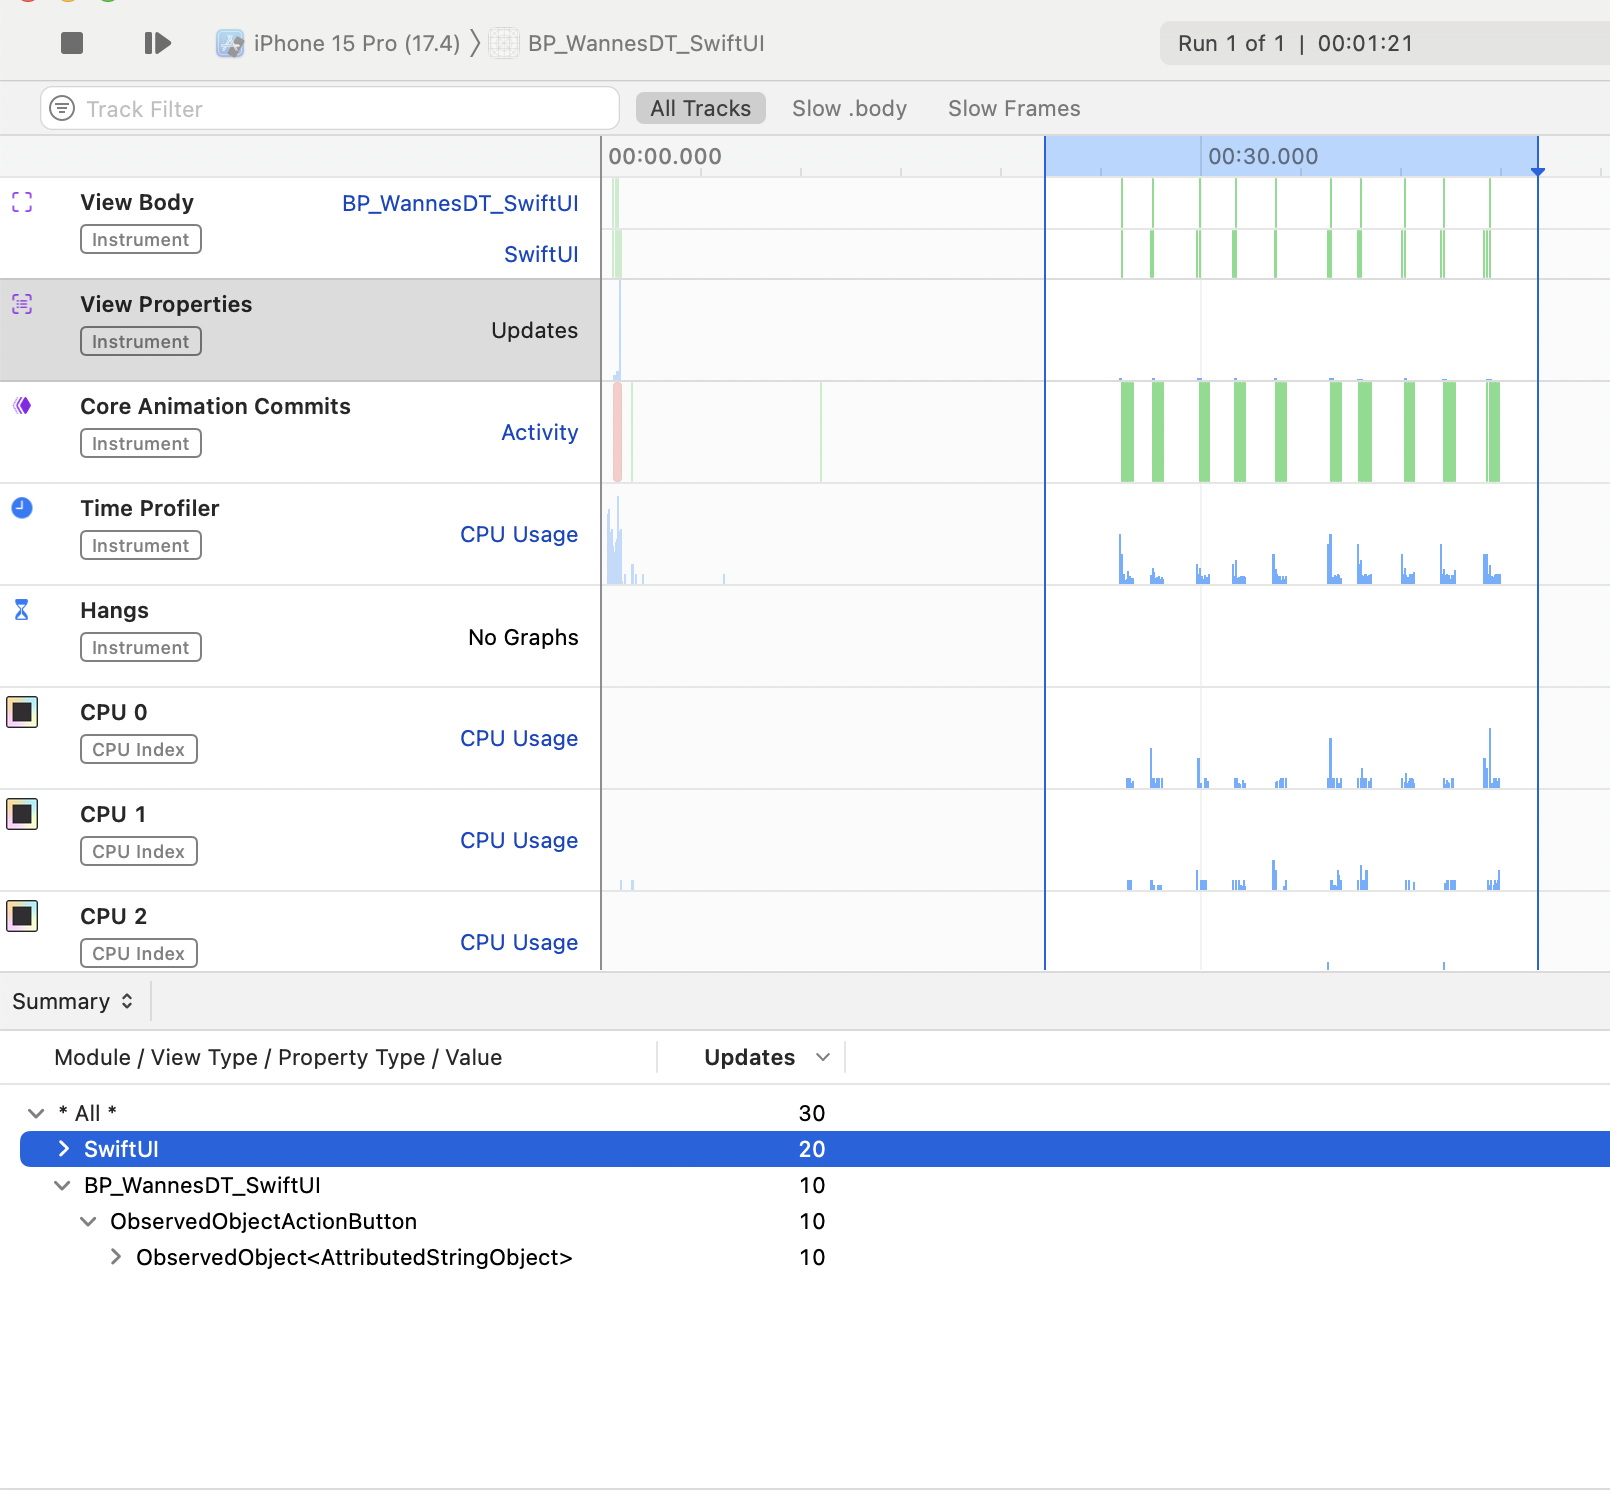
\includegraphics[width=0.7\textwidth]{bptest1_insubview/ObservableObjectButtonPressViewPropertyUpdates} 
    \caption{test2: Aantal keren dat de property's updaten bij het meervoudig toewijzigen van een ObservedObject}
    \label{fig:propertyUpdatesObservedObject1}
\end{figure}
\paragraph{Totale tijd gebruikt van de CPU}
\begin{figure}[H]
    \centering
    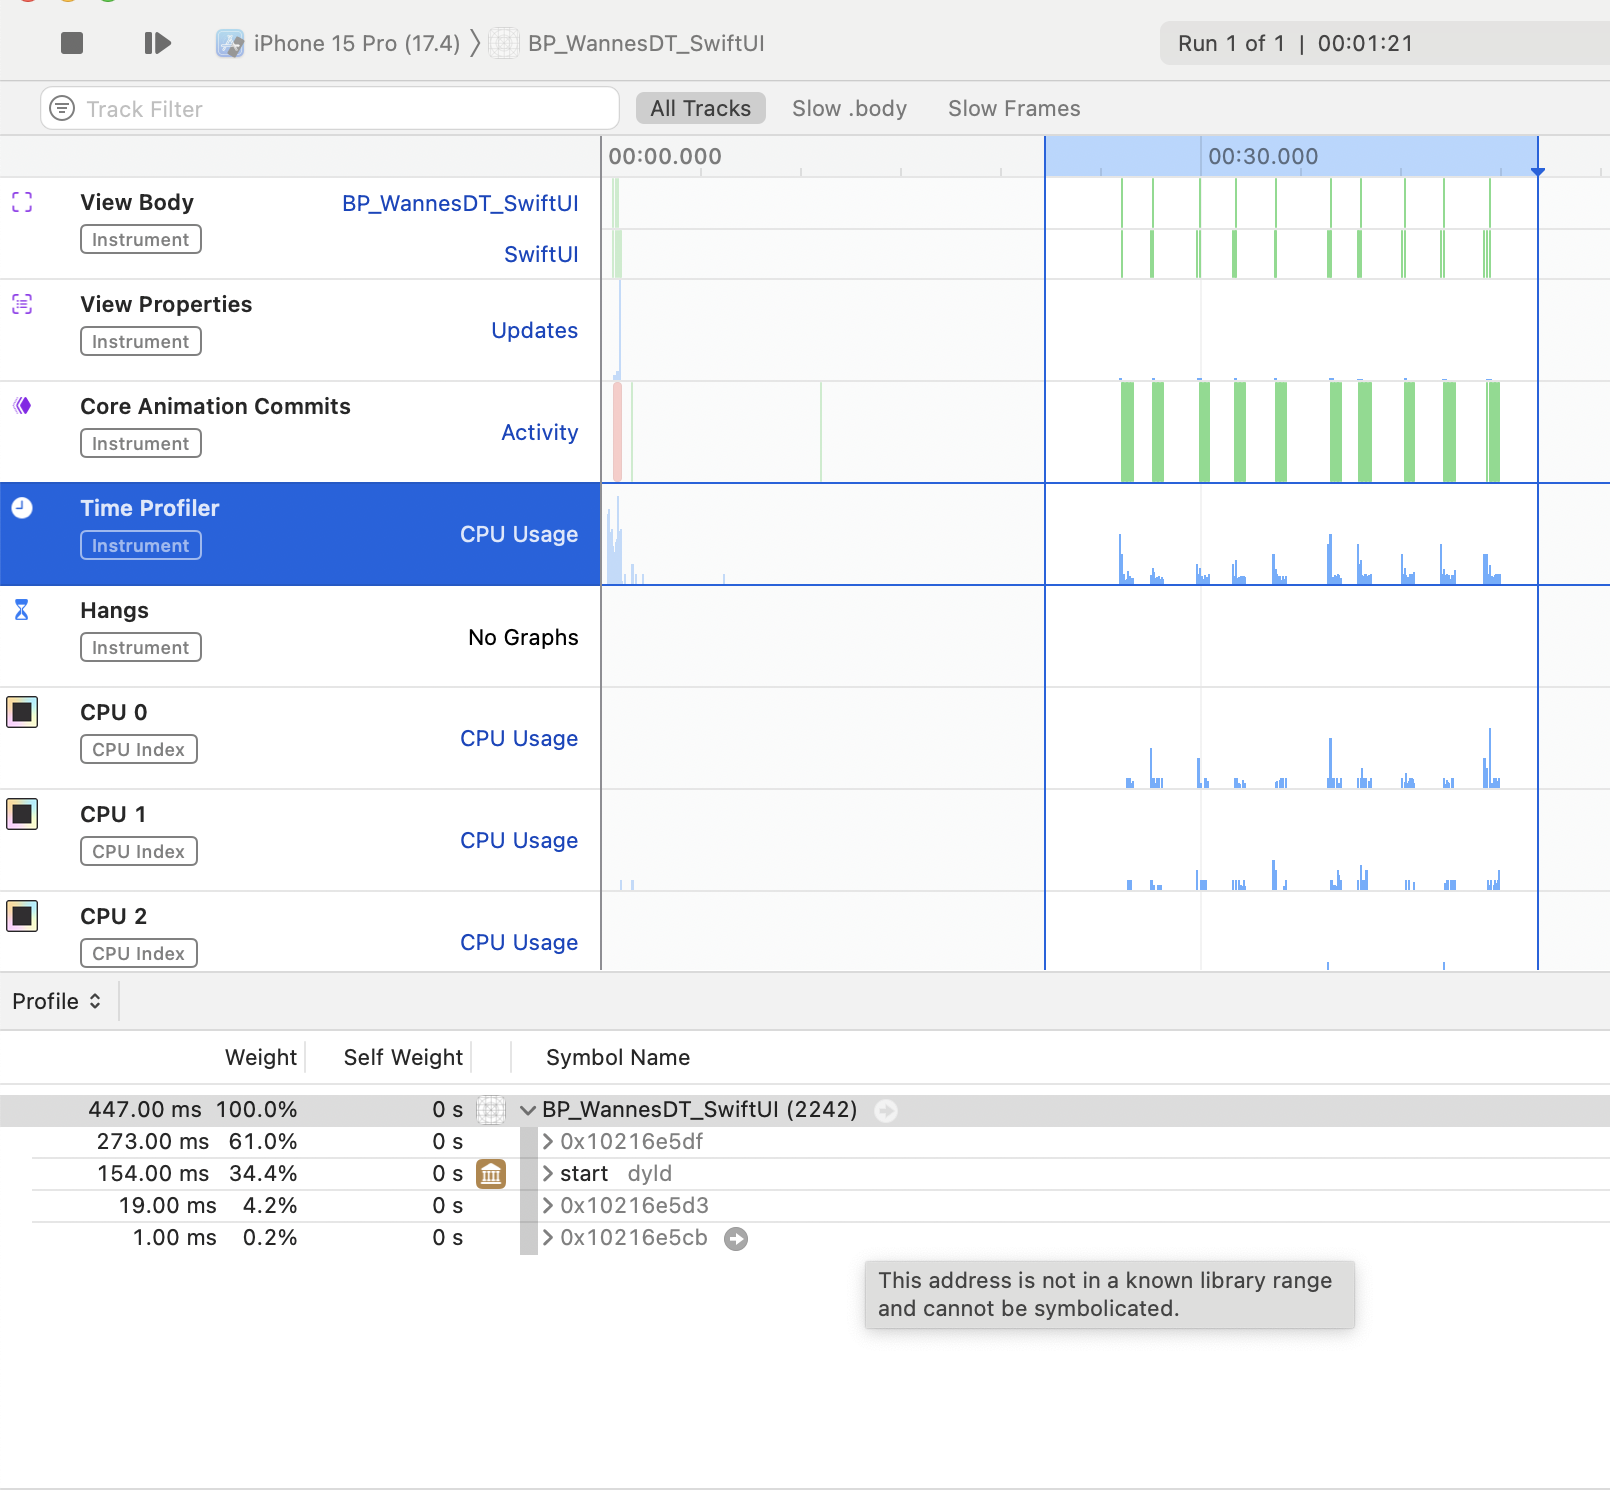
\includegraphics[width=0.7\textwidth]{bptest1_insubview/ObservableObjectButtonPressTotalCpuTime} 
    \caption{test2: De totale duratie die gebruikt is van de CPU bij het gebruik van ObservedObject}
    \label{fig:cpuUsageTimeObservedObject1}
\end{figure}
\paragraph{Last op de CPU}
\begin{figure}[H]
    \centering
    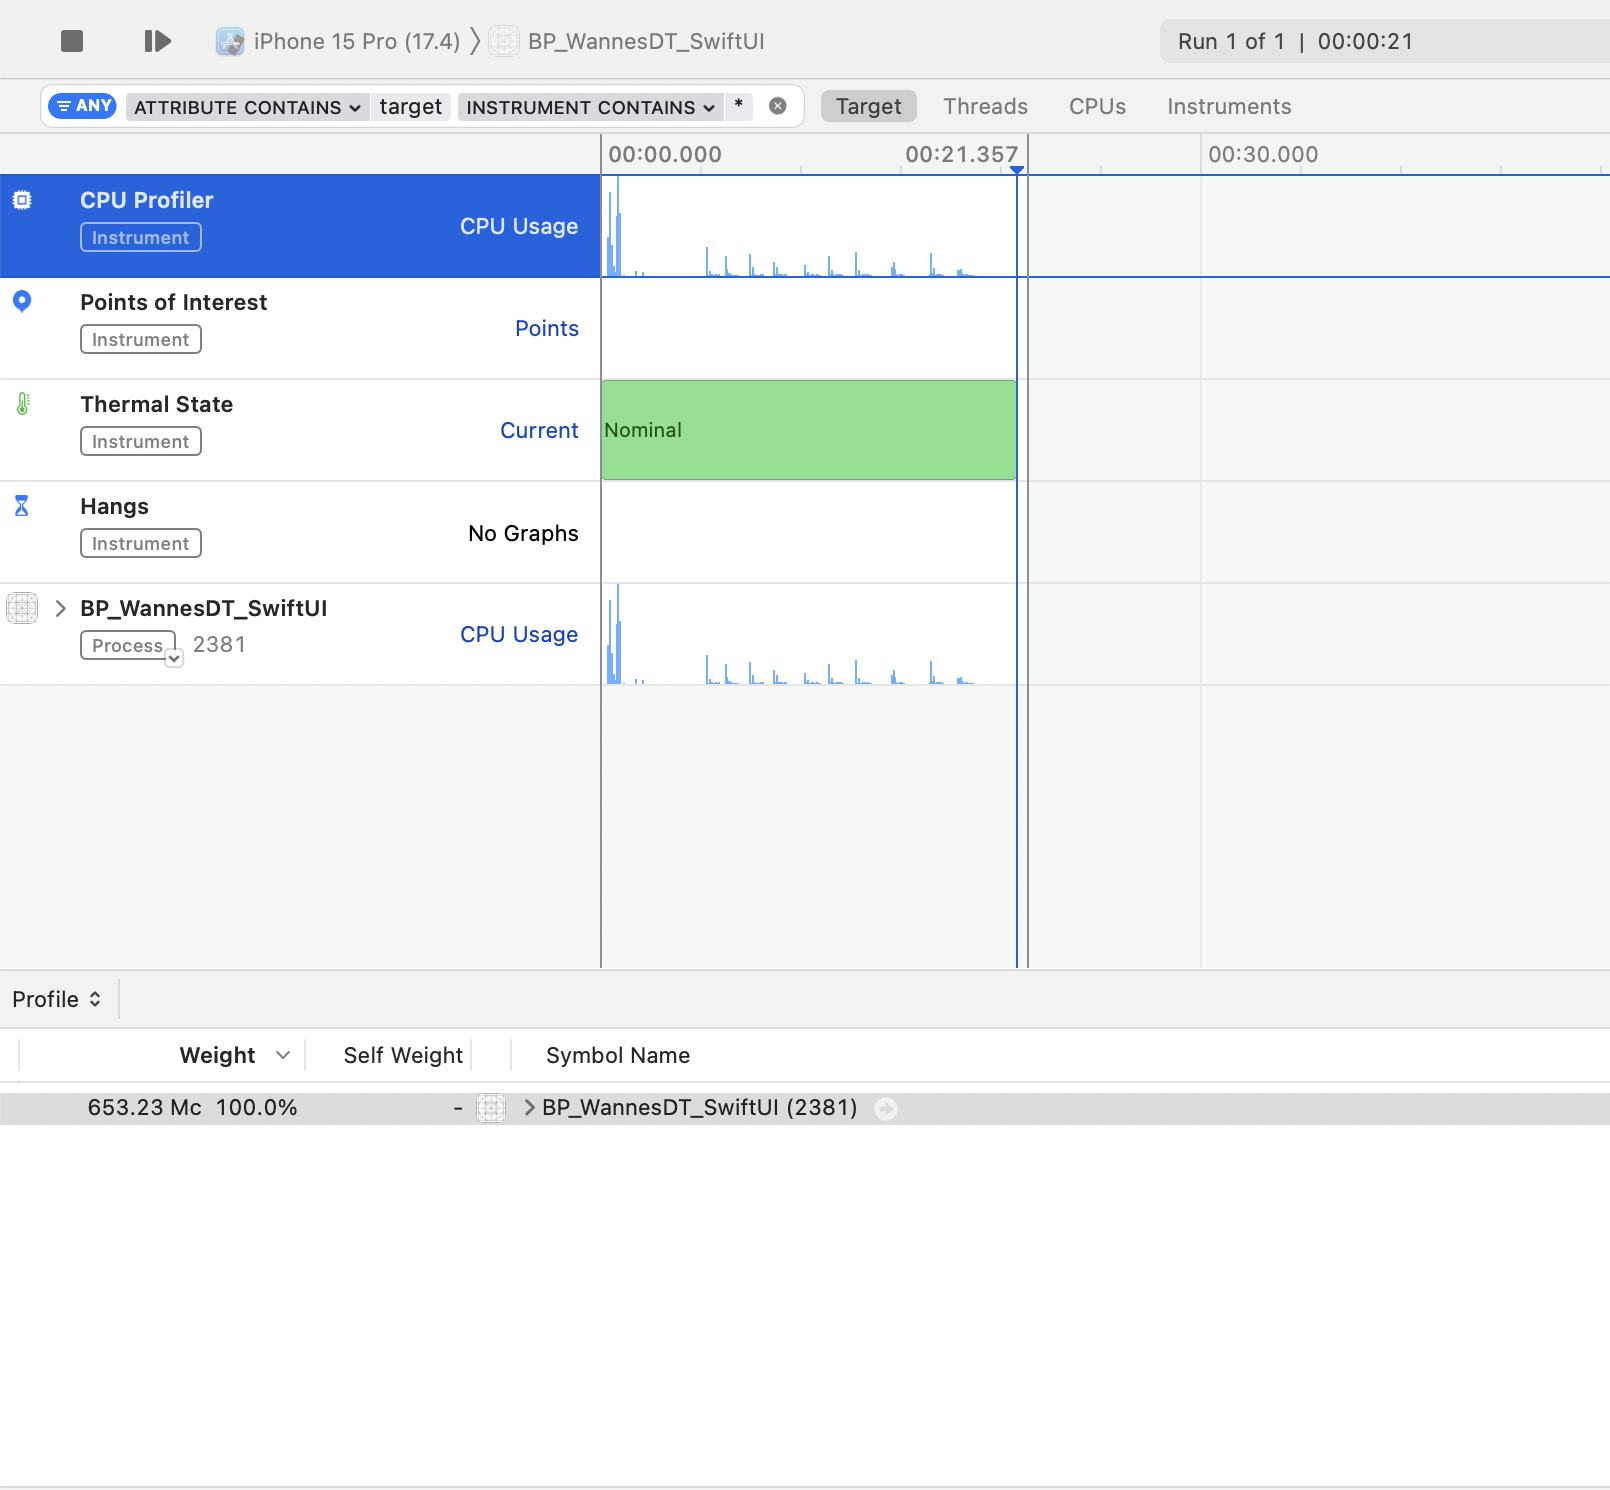
\includegraphics[width=0.7\textwidth]{bptest1_insubview/ObsrvableObjectButtonPressCpuUsage} 
    \caption{test2: De totale last van het opnieuw toewijzen van property's op de cpu bij het gebruik van ObservedObject}
    \label{fig:cpuWeightObservedObject1}
\end{figure}

\subsection{EnvironmentObject}
% EnvironmentObject test 1
\paragraph{View ververs aantal en ververs tijd}
\begin{figure}[H]
    \centering
    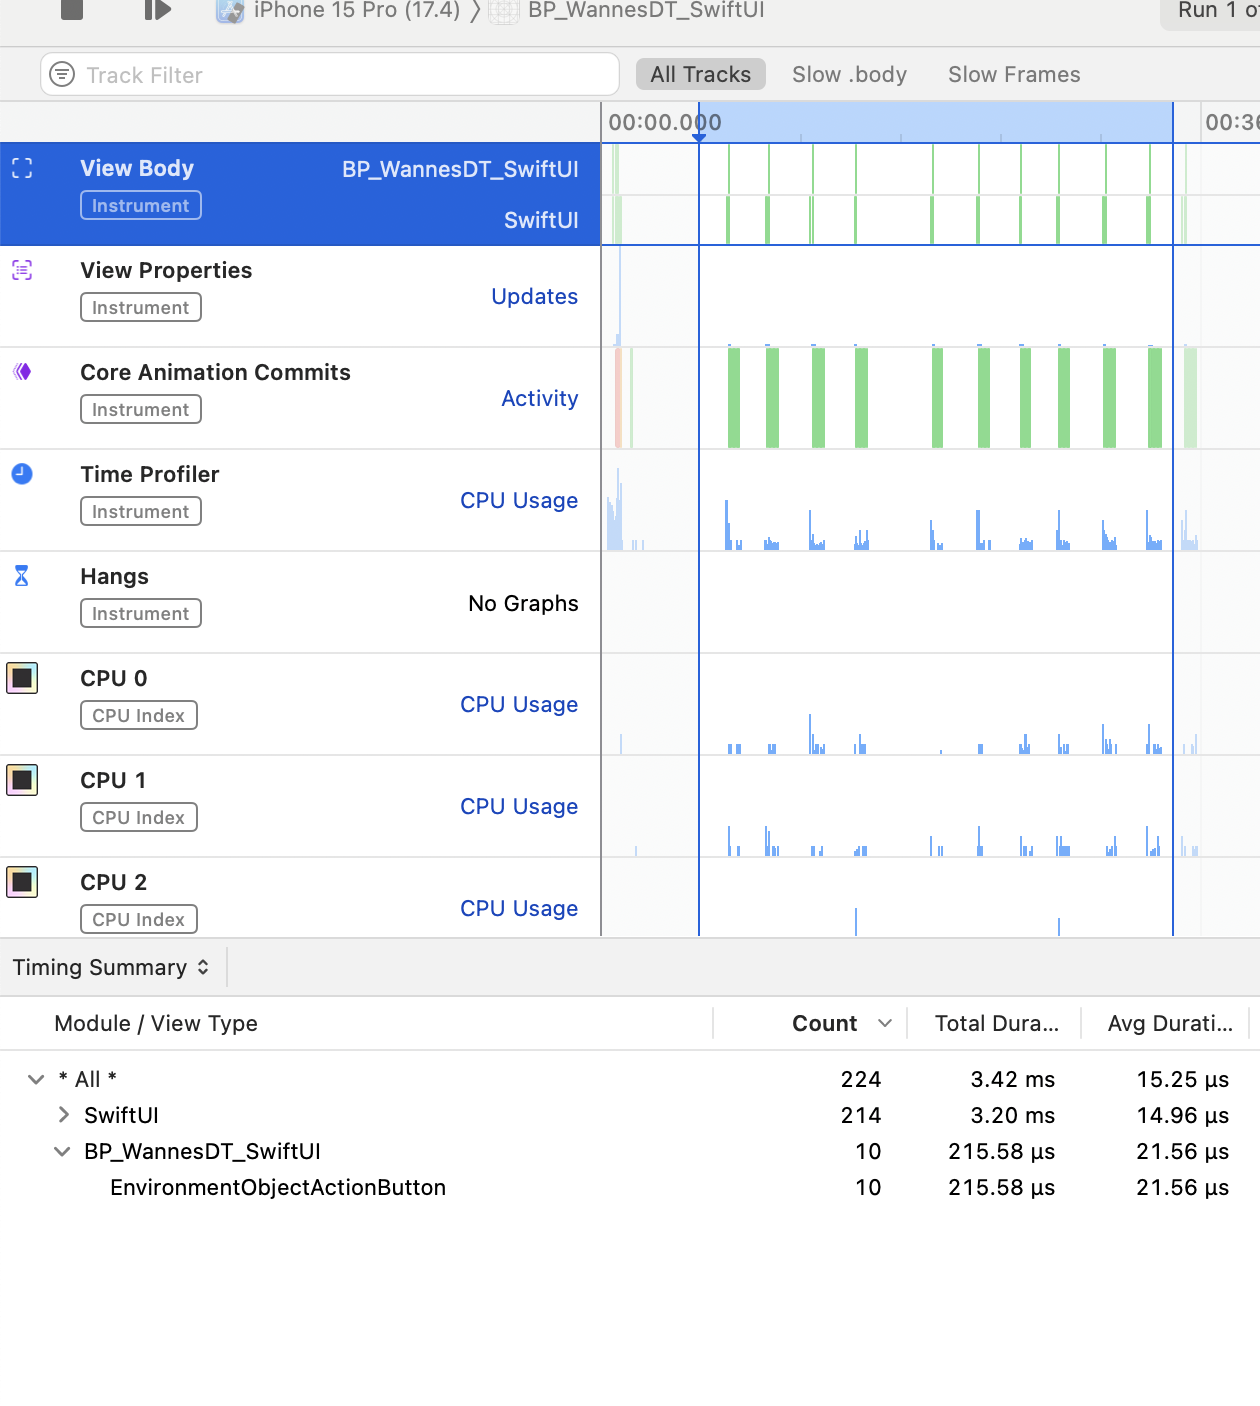
\includegraphics[width=0.7\textwidth]{bptest1_insubview/EnvironmentObjectButtonPressViewRefreshesAndTime} 
    \caption{test2: Aantal keren dat de view refreshed en gemiddelde duratie bij het meervoudig toewijzigen van een EnvironmentObject}
    \label{fig:viewRefresheEnvironmentObject1}
\end{figure}
\paragraph{Aantal updates van property's}
\begin{figure}[H]
    \centering
    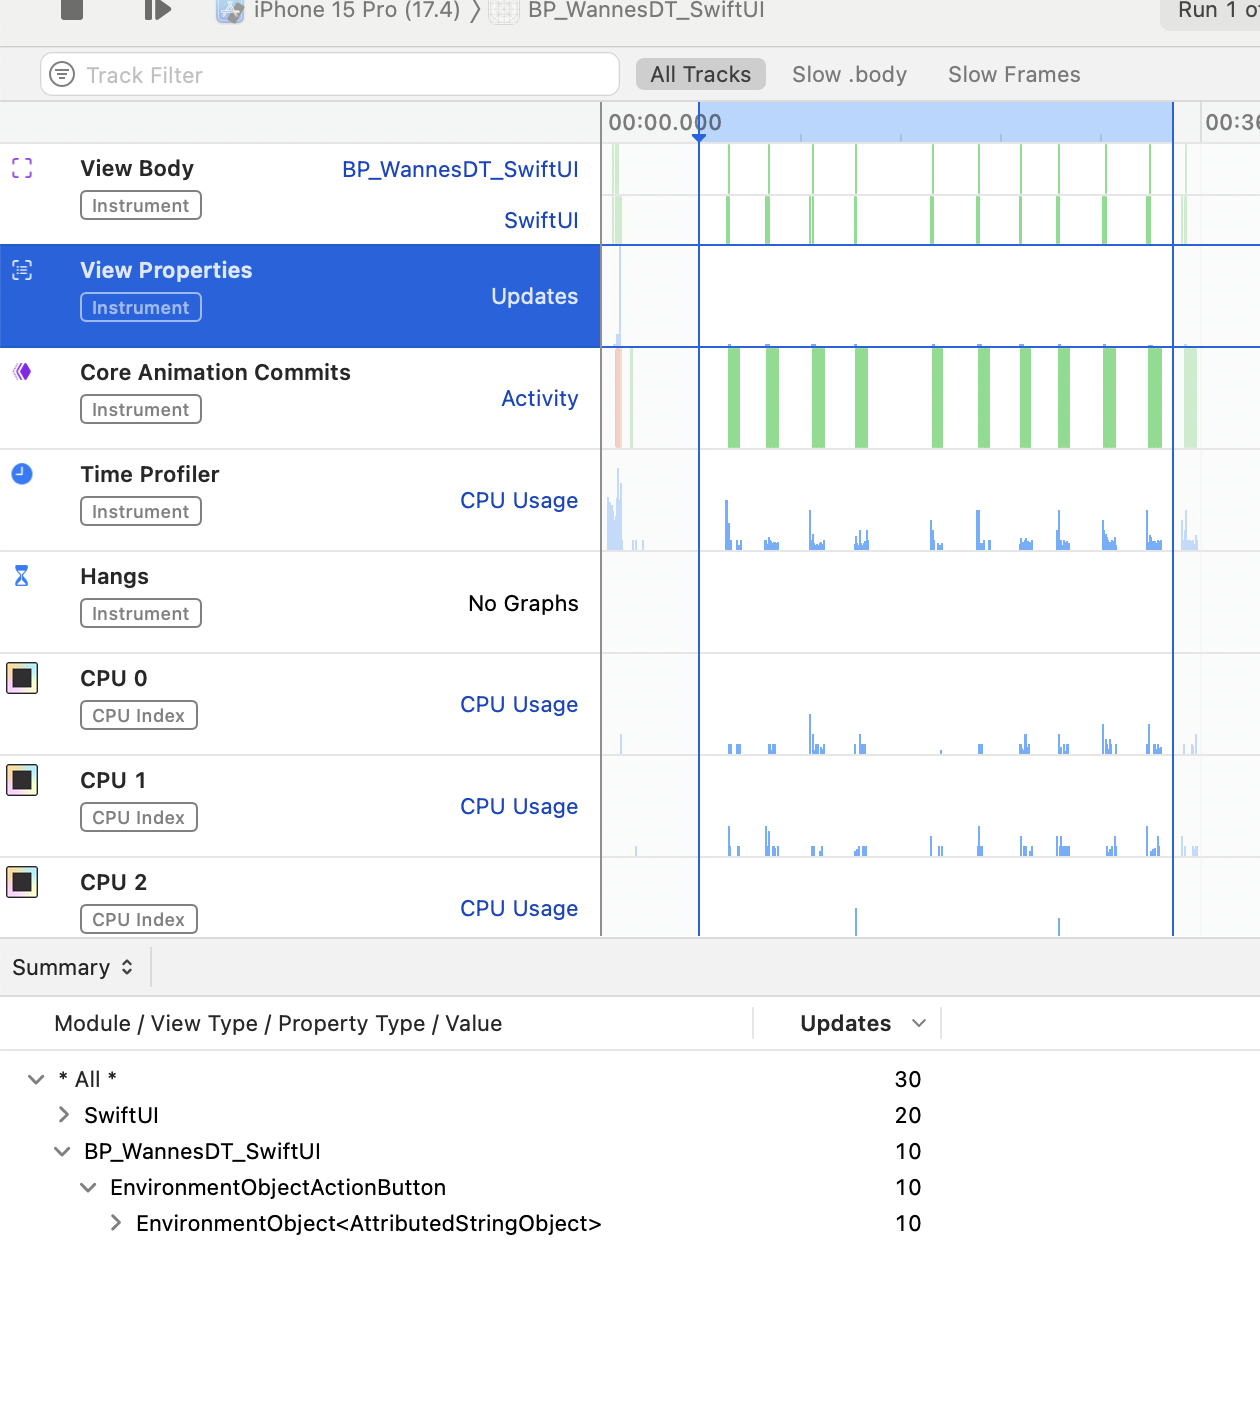
\includegraphics[width=0.7\textwidth]{bptest1_insubview/EnvironnmentObjectButtonPressViewPropertyUpdates} 
    \caption{test2: Aantal keren dat de property's updaten bij het meervoudig toewijzigen van een EnvironmentObject}
    \label{fig:propertyUpdatesEnvironmentObject1}
\end{figure}
\paragraph{Totale tijd gebruikt van de CPU}
\begin{figure}[H]
    \centering
    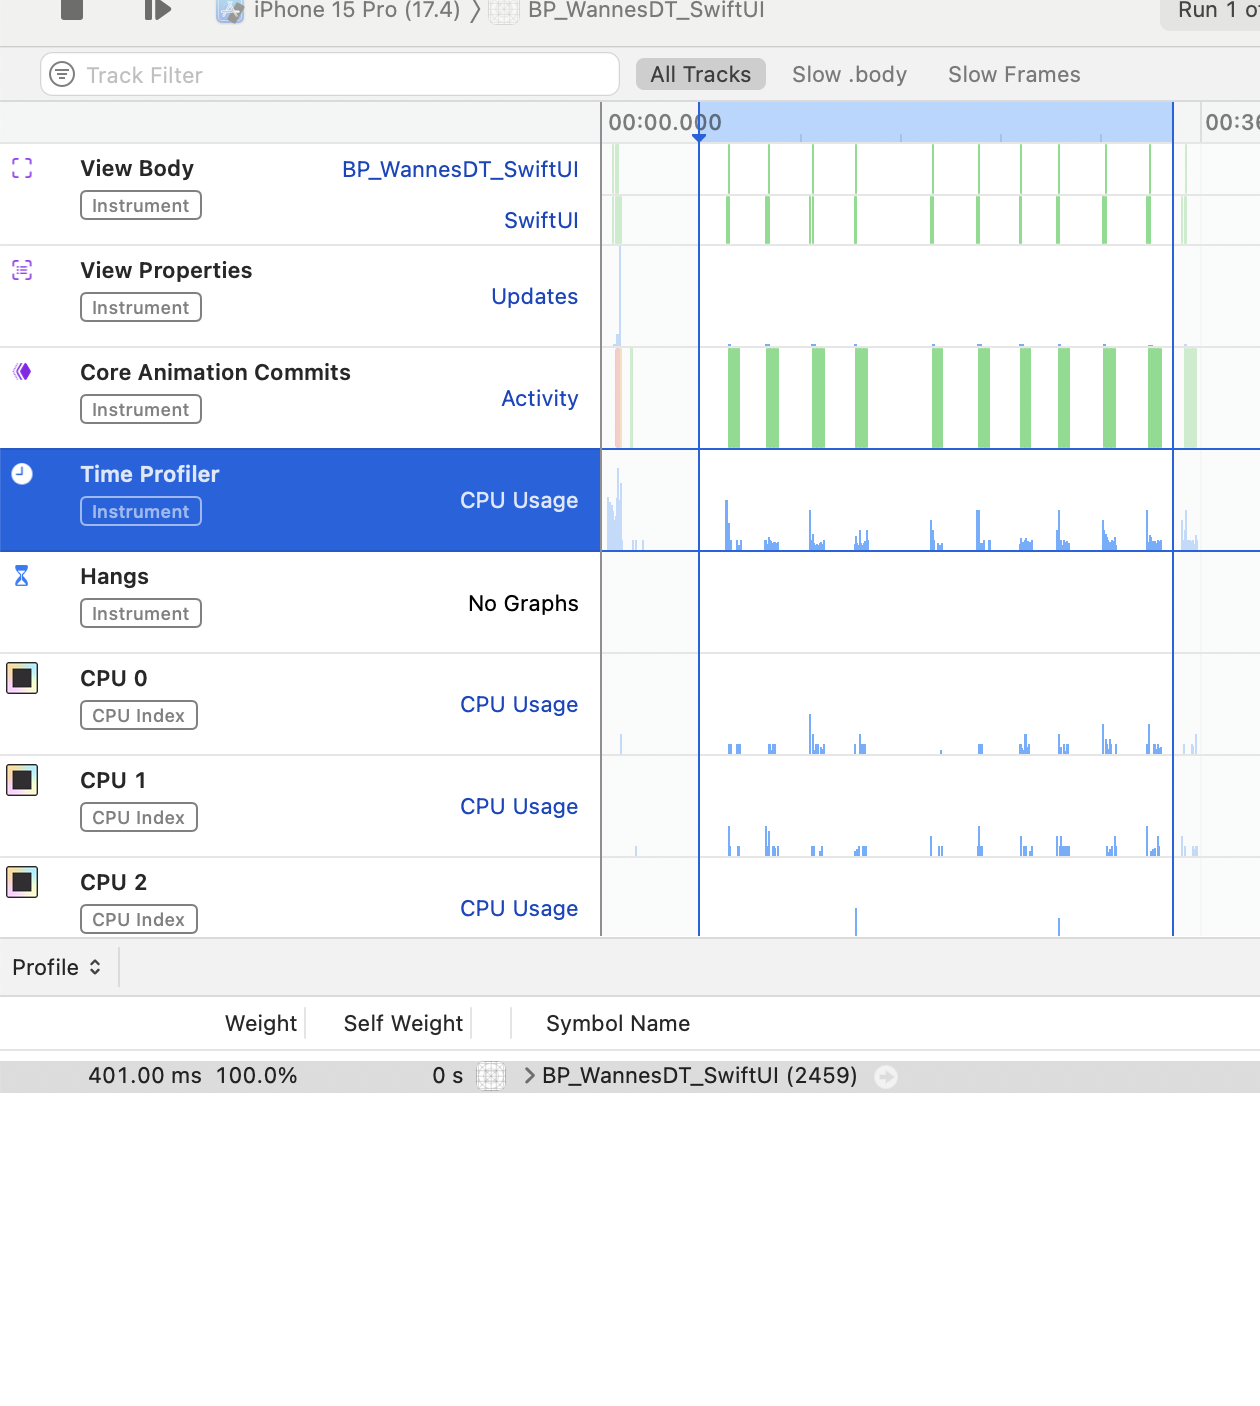
\includegraphics[width=0.7\textwidth]{bptest1_insubview/EnvironmentObjectButtonPressTotalCpuTime} 
    \caption{test2: De totale duratie die gebruikt is van de CPU bij het gebruik van EnvironmentObject}
    \label{fig:cpuUsageTimeEnvironmentObject1}
\end{figure}
\paragraph{Last op de CPU}
\begin{figure}[H]
    \centering
    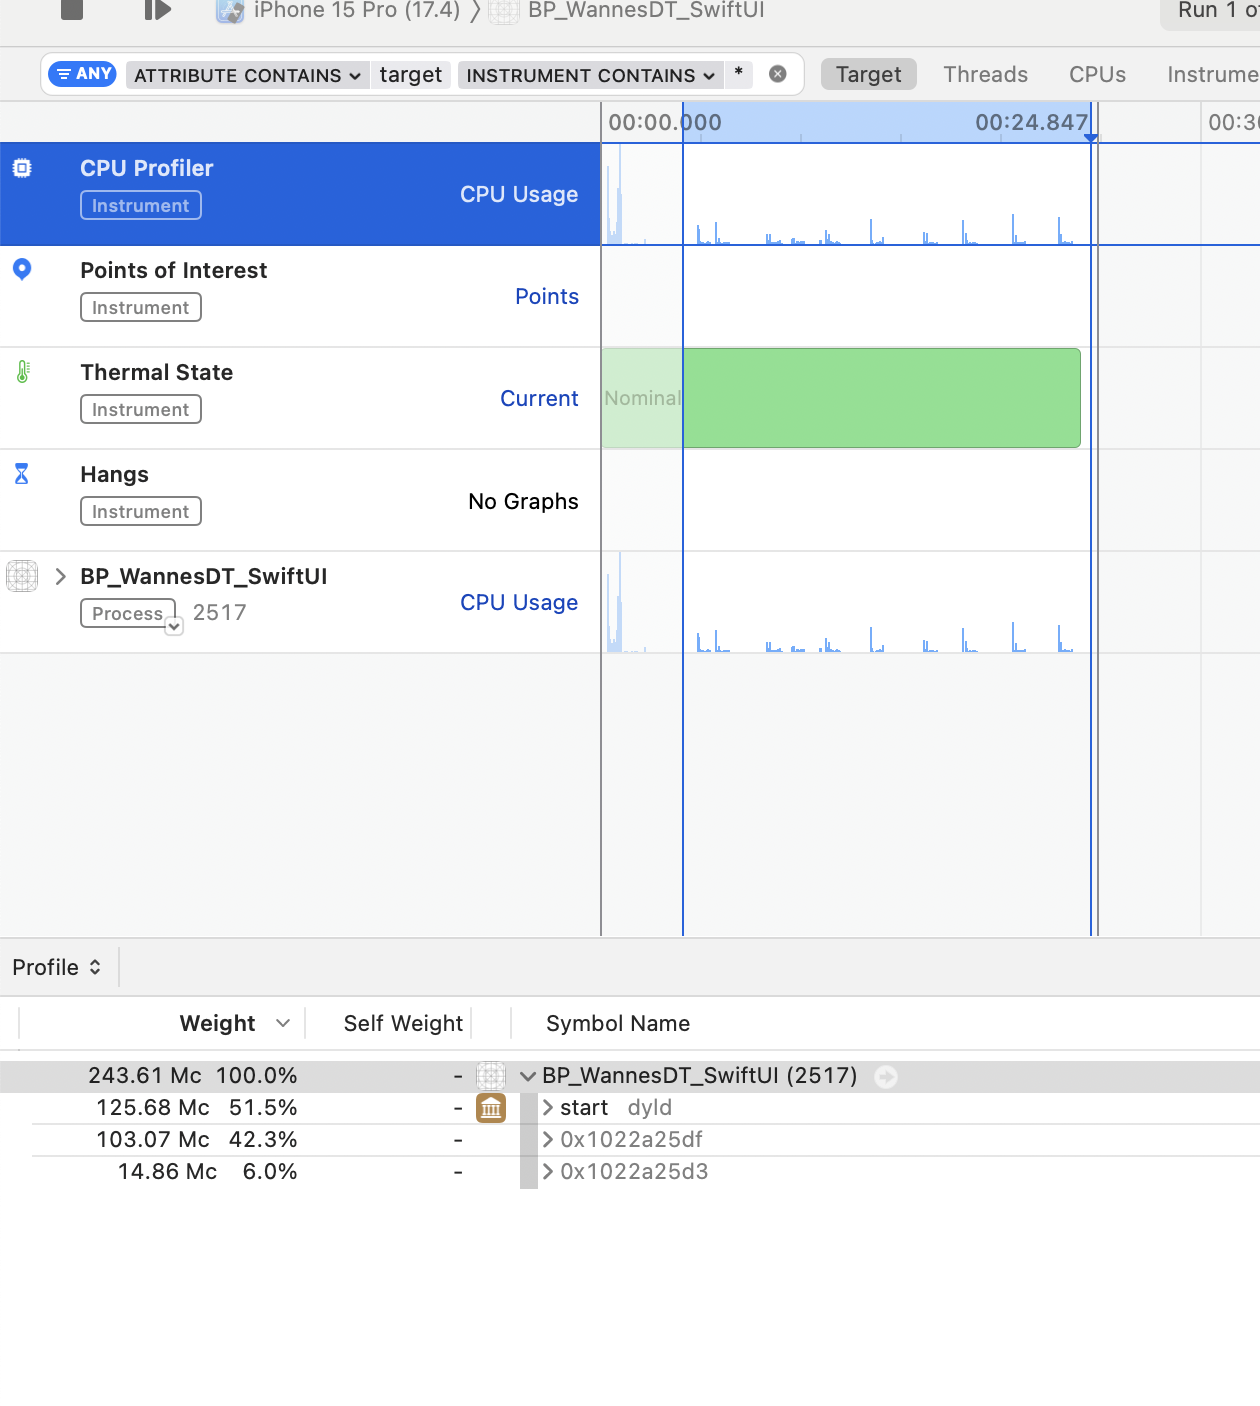
\includegraphics[width=0.7\textwidth]{bptest1_insubview/EnvironmentObjectButtonPressCpuUsage} 
    \caption{test2: De totale last van het opnieuw toewijzen van property's op de cpu bij het gebruik van EnvironmentObject}
    \label{fig:cpuWeightEnvironmentObject1}
\end{figure}

\section{Test3: Dataoverdracht naar meerdere subview's met lazyLists}

\subsection{Binding}
\paragraph{View ververs aantal en ververs tijd}
\begin{figure}[H]
    \centering
    \includegraphics[width=0.7\textwidth]{BPtest2_lazy/BindingViewRefreshes} 
    \caption{test3: Aantal keren dat de view refreshed en gemiddelde duratie bij het meervoudig toewijzigen van een binding}
    \label{fig:viewRefreshesBinding2}
\end{figure}
\paragraph{Aantal updates van property's}
\begin{figure}[H]
    \centering
    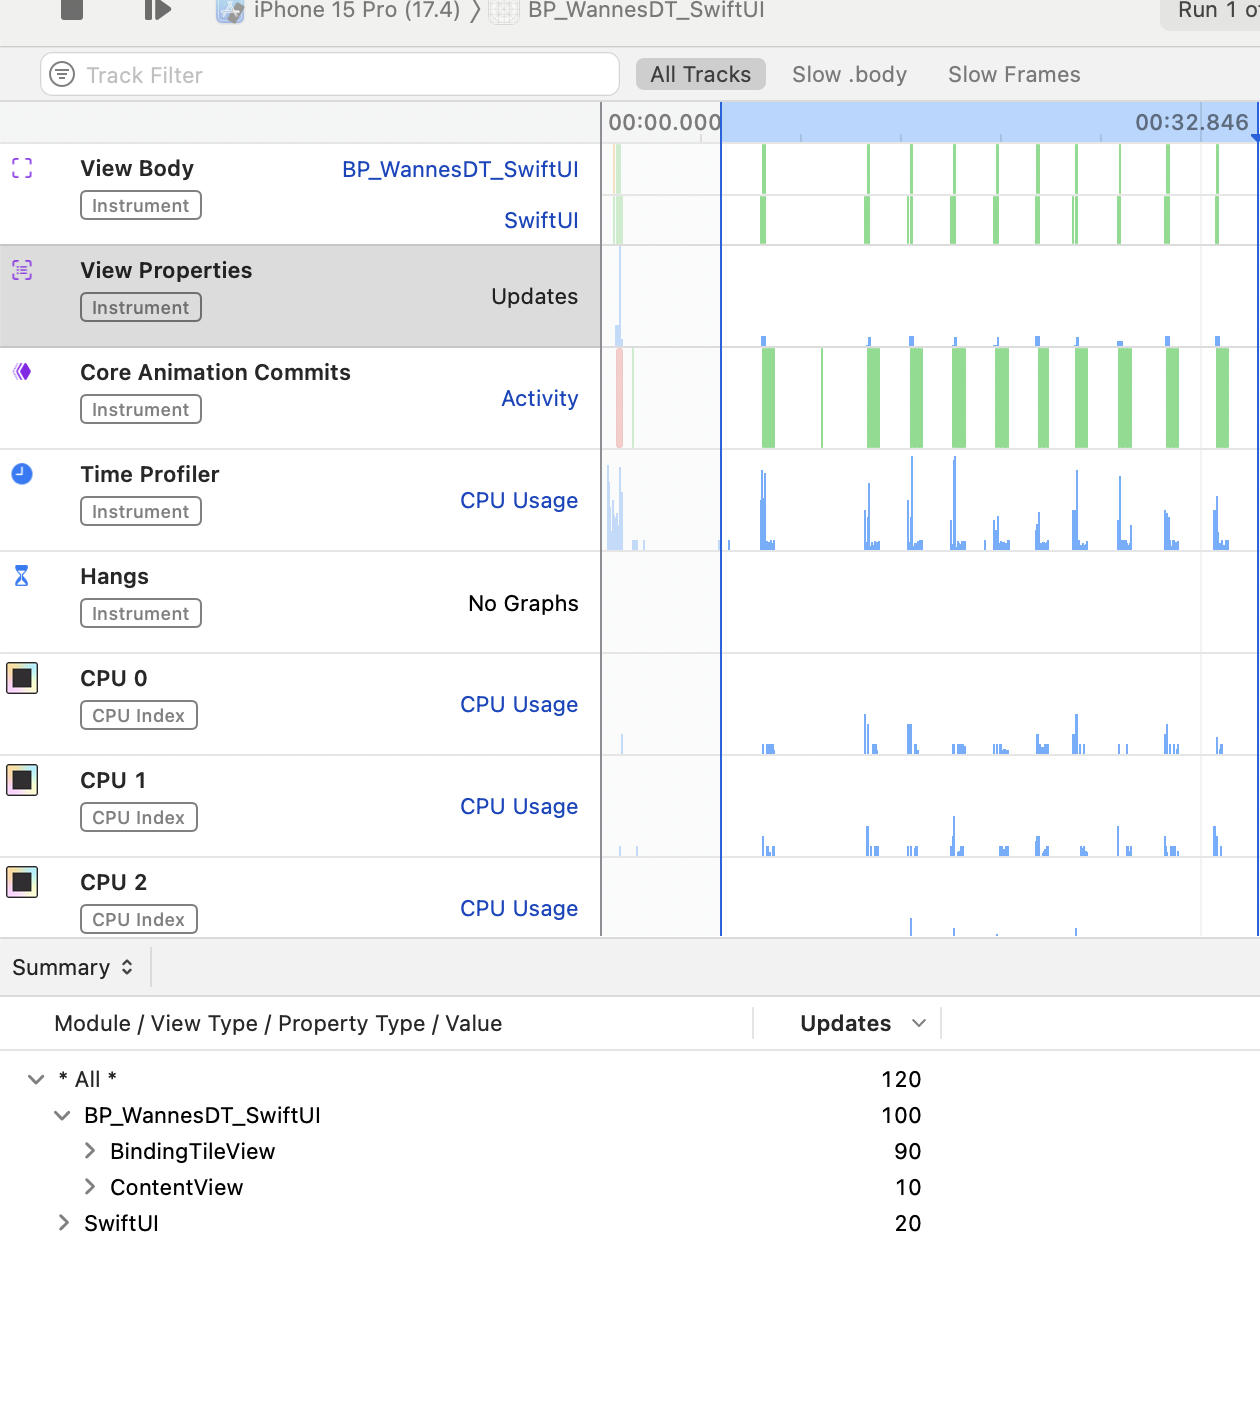
\includegraphics[width=0.7\textwidth]{BPtest2_lazy/BindingPropertyUpdates} 
    \caption{test3: Aantal keren dat de property's updaten bij het meervoudig toewijzigen van een binding}
    \label{fig:propertyUpdatesBinding2}
\end{figure}
\paragraph{Totale tijd gebruikt van de CPU}
\begin{figure}[H]
    \centering
    \includegraphics[width=0.7\textwidth]{BPtest2_lazy/BindingTotalCpuTime} 
    \caption{test3: De totale duratie die gebruikt is van de CPU bij het gebruik van bindings}
    \label{fig:cpuUsageTimeBinding2}
\end{figure}
\paragraph{Last op de CPU}
\begin{figure}[H]
    \centering
    \includegraphics[width=0.7\textwidth]{BPtest2_lazy/BindingCpuWeight} 
    \caption{test3: De totale last van het opnieuw toewijzen van property's op de cpu bij het gebruik van bindings}
    \label{fig:cpuWeightBinding2}
\end{figure}

% Observable test 2
\subsection{Observable}
\paragraph{View ververs aantal en ververs tijd}
\begin{figure}[H]
    \centering
    \includegraphics[width=0.7\textwidth]{BPtest2_lazy/ObservableViewRefreshes} 
    \caption{test3: Aantal keren dat de view refreshed en gemiddelde duratie bij het meervoudig toewijzigen van een Observable}
    \label{fig:viewRefreshesObservable2}
\end{figure}
\paragraph{Aantal updates van property's}
\begin{figure}[H]
    \centering
    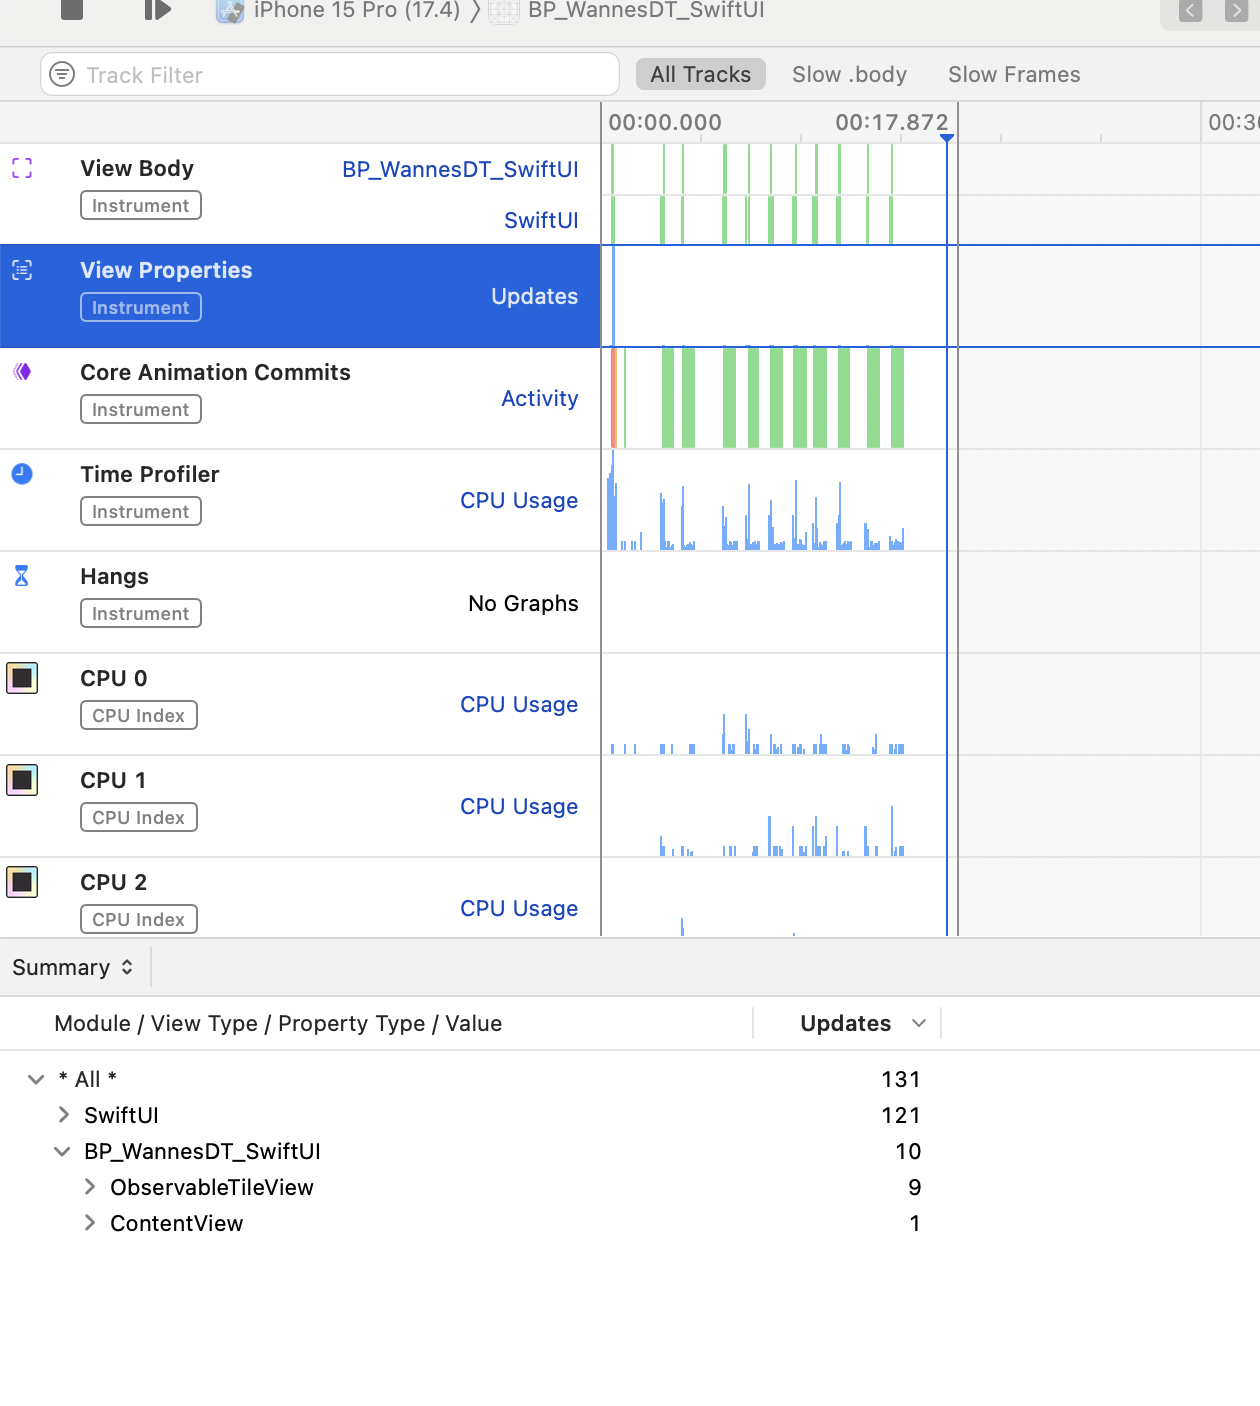
\includegraphics[width=0.7\textwidth]{BPtest2_lazy/ObservablePropertyUpdates} 
    \caption{test3: Aantal keren dat de property's updaten bij het meervoudig toewijzigen van een Observable}
    \label{fig:propertyUpdatesObservable2}
\end{figure}
\paragraph{Totale tijd gebruikt van de CPU}
\begin{figure}[H]
    \centering
    \includegraphics[width=0.7\textwidth]{BPtest2_lazy/ObservableTotalCpuTime} 
    \caption{test3: De totale duratie die gebruikt is van de CPU bij het gebruik van Observable's}
    \label{fig:cpuUsageTimeObservable2}
\end{figure}
\paragraph{Last op de CPU}
\begin{figure}[H]
    \centering
    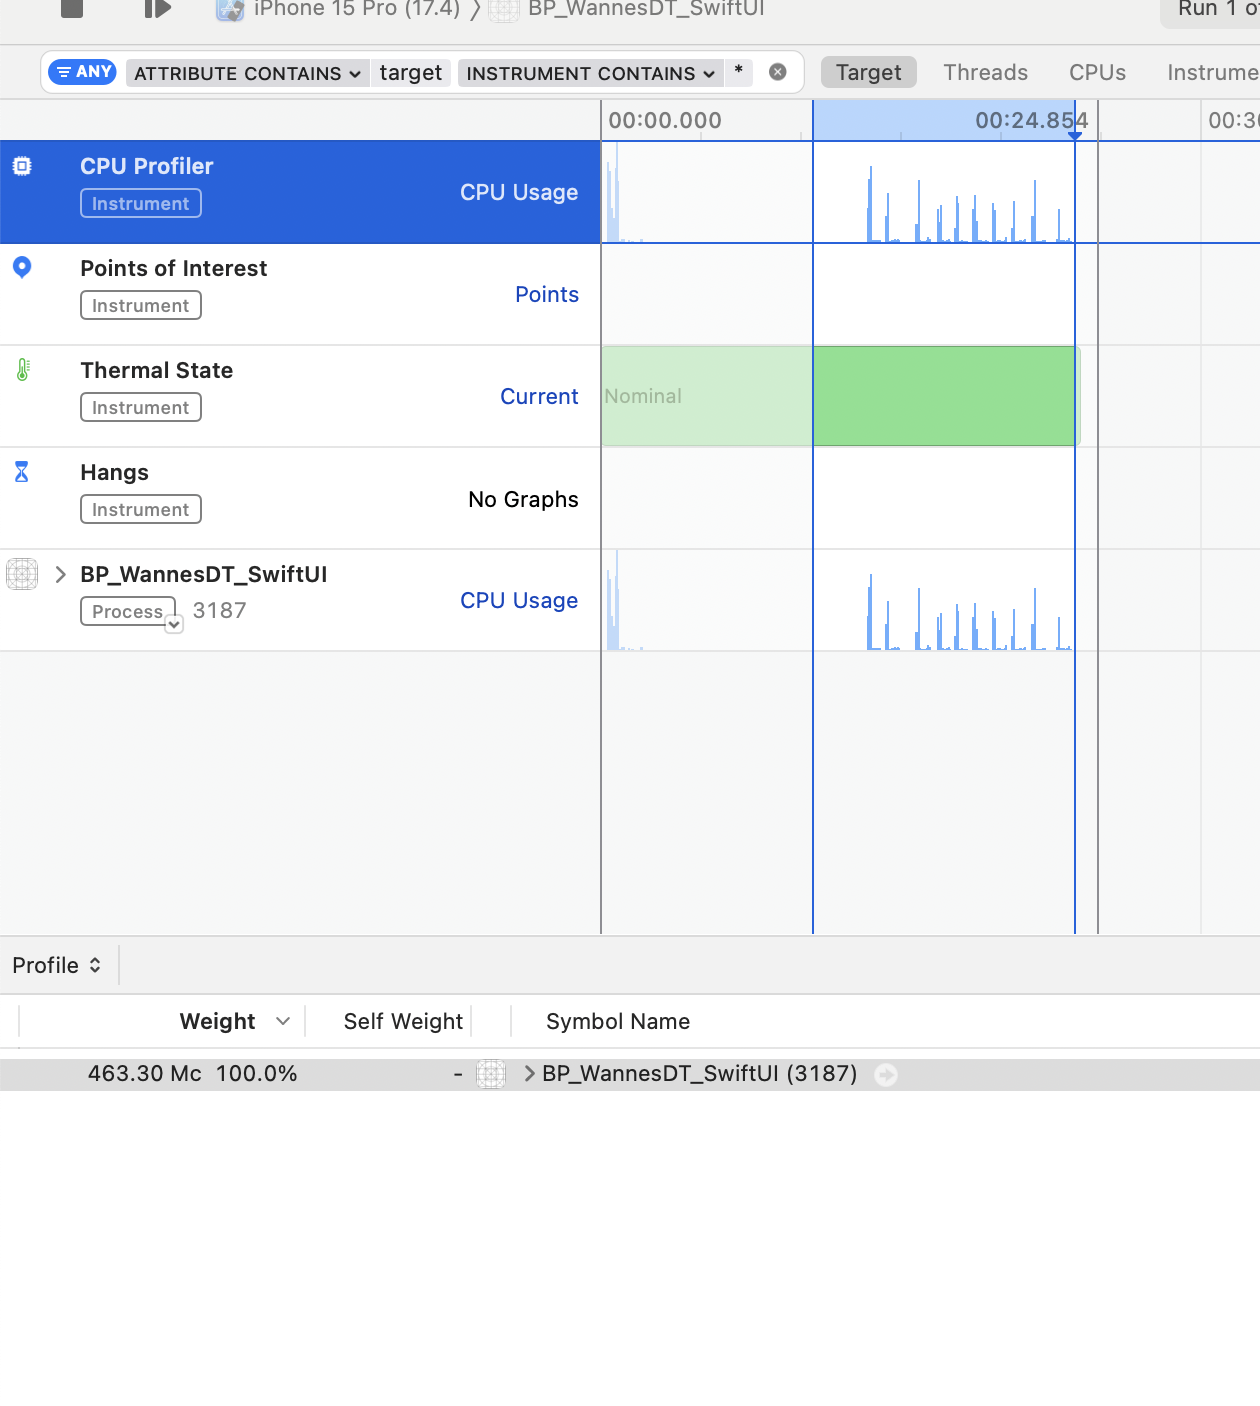
\includegraphics[width=0.7\textwidth]{BPtest2_lazy/ObservableCpuWieght} 
    \caption{test3: De totale last van het opnieuw toewijzen van property's op de cpu bij het gebruik van Observable's}
    \label{fig:cpuWeightObservable2}
\end{figure}

% ObservedObject test 2
\subsection{ObservedObject}
\paragraph{View ververs aantal en ververs tijd}
\begin{figure}[H]
    \centering
    \includegraphics[width=0.7\textwidth]{BPtest2_lazy/ObservedObjectViewRefreshes} 
    \caption{test3: Aantal keren dat de view refreshed en gemiddelde duratie bij het meervoudig toewijzigen van een ObservedObject}
    \label{fig:viewRefreshesObservedObject2}
\end{figure}
\paragraph{Aantal updates van property's}
\begin{figure}[H]
    \centering
    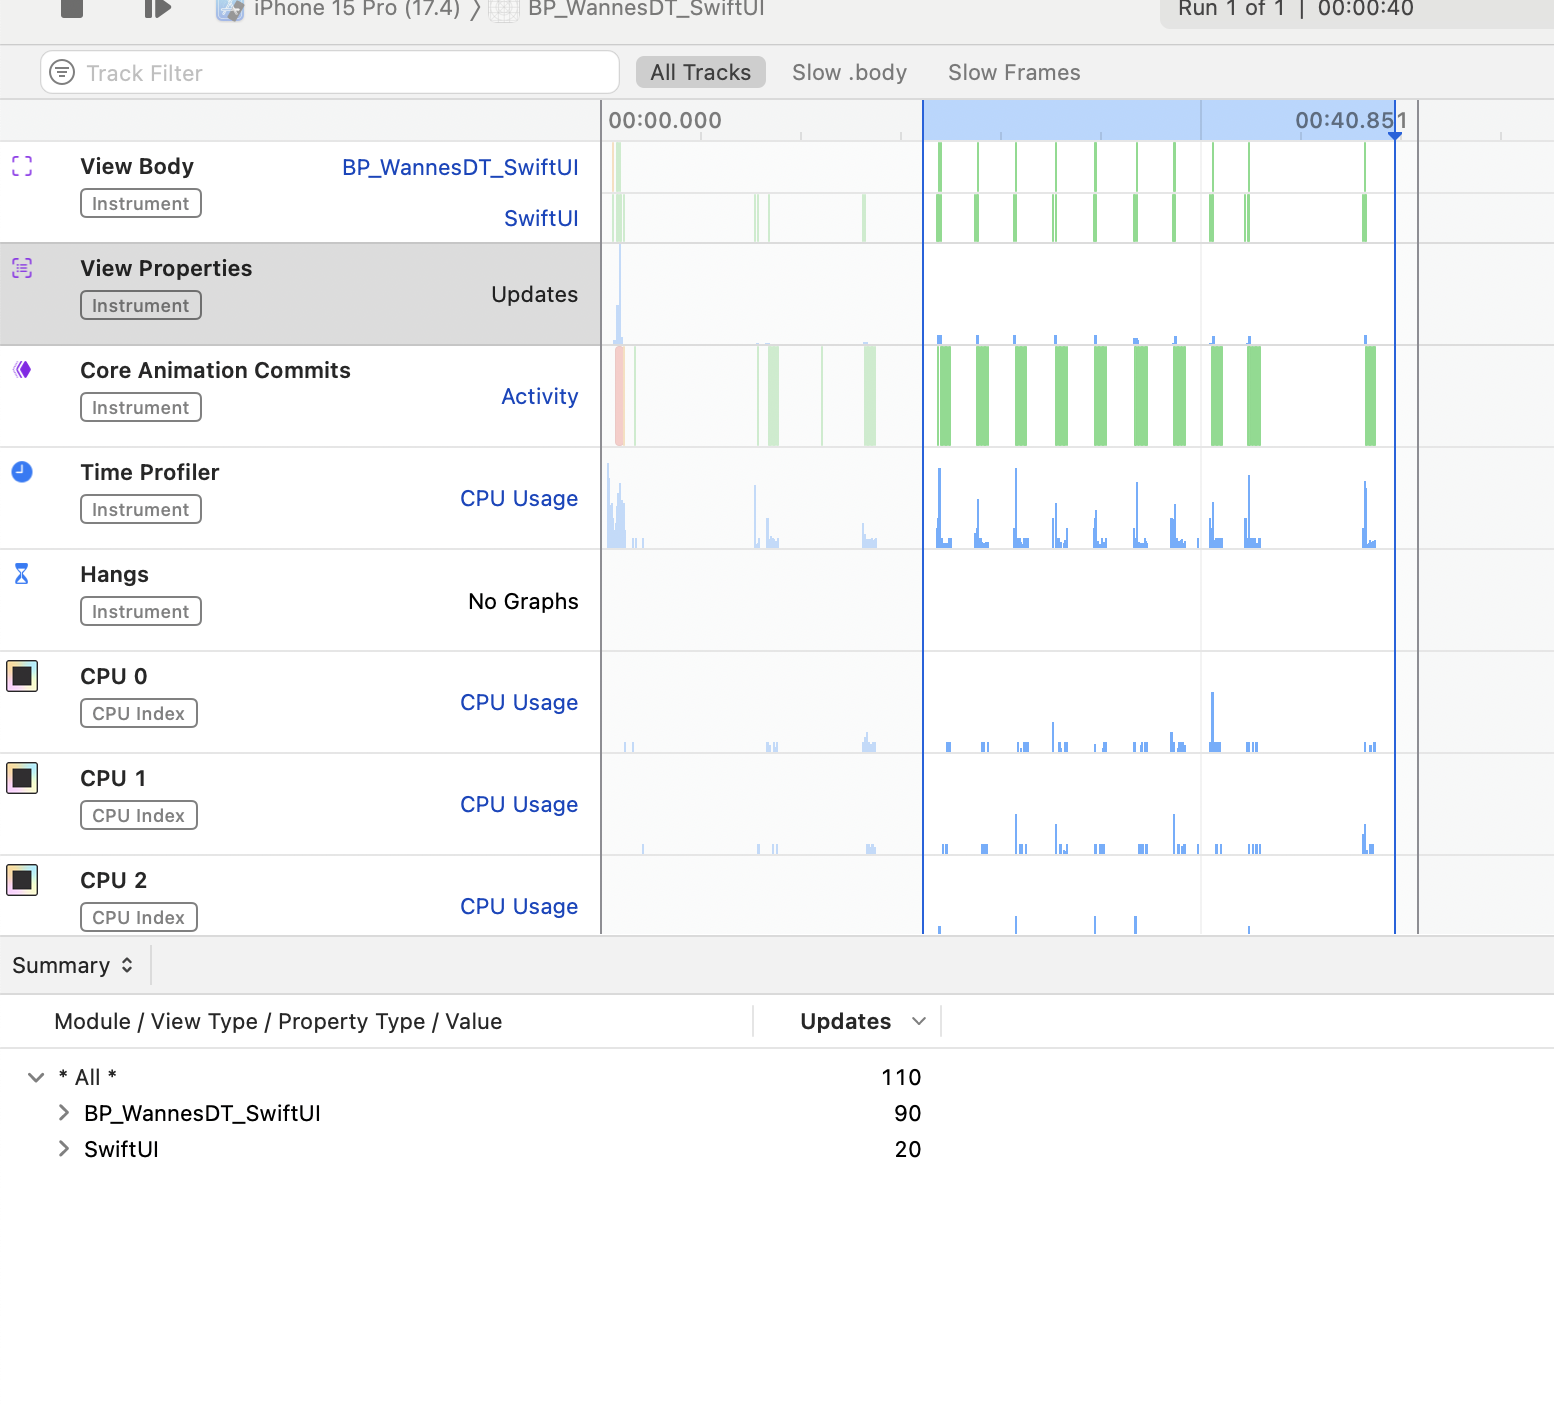
\includegraphics[width=0.7\textwidth]{BPtest2_lazy/ObservedObjectPropertyUpdates} 
    \caption{test3: Aantal keren dat de property's updaten bij het meervoudig toewijzigen van een ObservedObject}
    \label{fig:propertyUpdatesObservedObject2}
\end{figure}
\paragraph{Totale tijd gebruikt van de CPU}
\begin{figure}[H]
    \centering
    \includegraphics[width=0.7\textwidth]{BPtest2_lazy/ObservedObjectTotalCpuTime} 
    \caption{test3: De totale duratie die gebruikt is van de CPU bij het gebruik van ObservedObject's}
    \label{fig:cpuUsageTimeObservedObject2}
\end{figure}
\paragraph{Last op de CPU}
\begin{figure}[H]
    \centering
    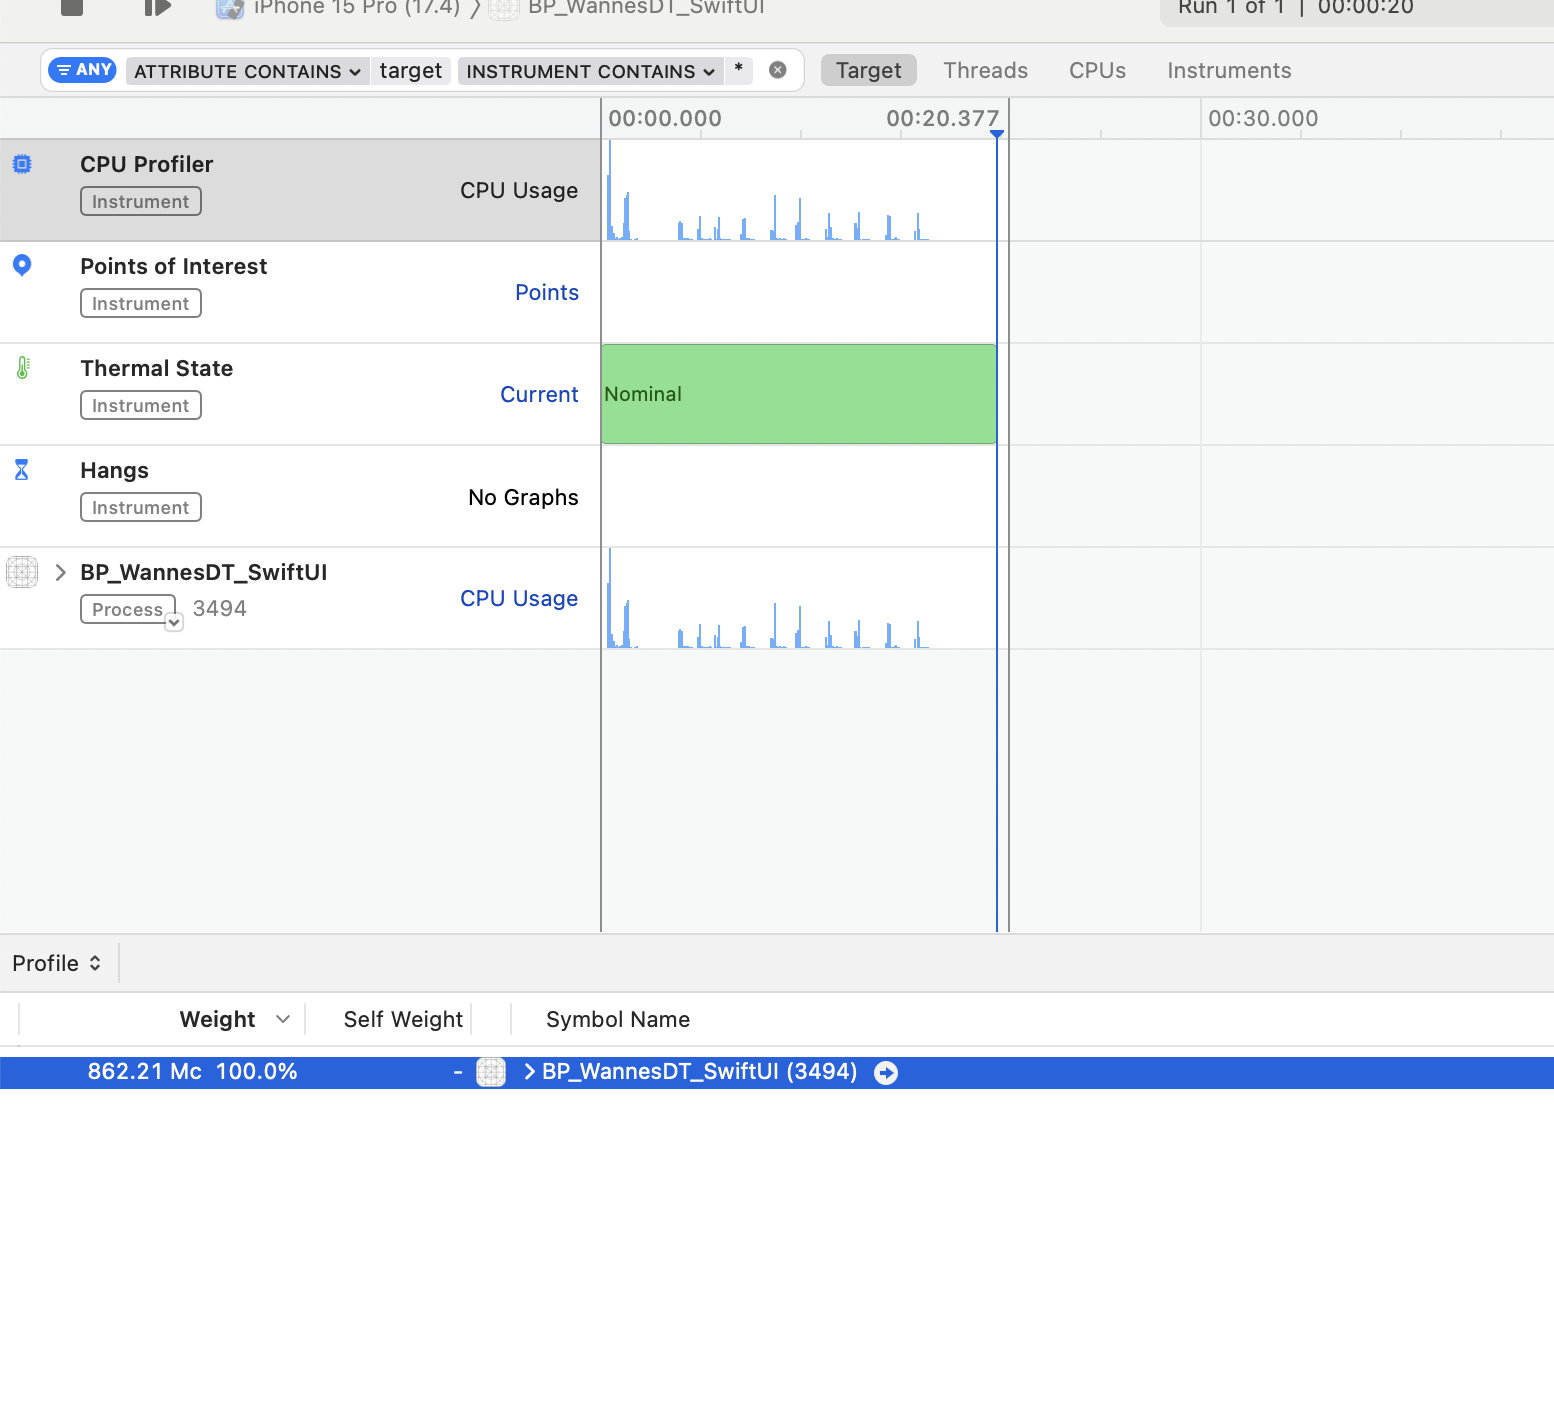
\includegraphics[width=0.7\textwidth]{BPtest2_lazy/ObservedObjectCpuWieght} 
    \caption{test3: De totale last van het opnieuw toewijzen van property's op de cpu bij het gebruik van ObservedObject's}
    \label{fig:cpuWeightObservedObject2}
\end{figure}

% EnvironmentObject test 2
\subsection{EnvironmentObject}
\paragraph{View ververs aantal en ververs tijd}
\begin{figure}[H]
    \centering
    \includegraphics[width=0.7\textwidth]{BPtest2_lazy/EnvironmentObjectViewRefreshes} 
    \caption{test3: Aantal keren dat de view refreshed en gemiddelde duratie bij het meervoudig toewijzigen van een EnvironmentObject}
    \label{fig:viewRefreshesEnvironmentObject2}
\end{figure}
\paragraph{Aantal updates van property's}
\begin{figure}[H]
    \centering
    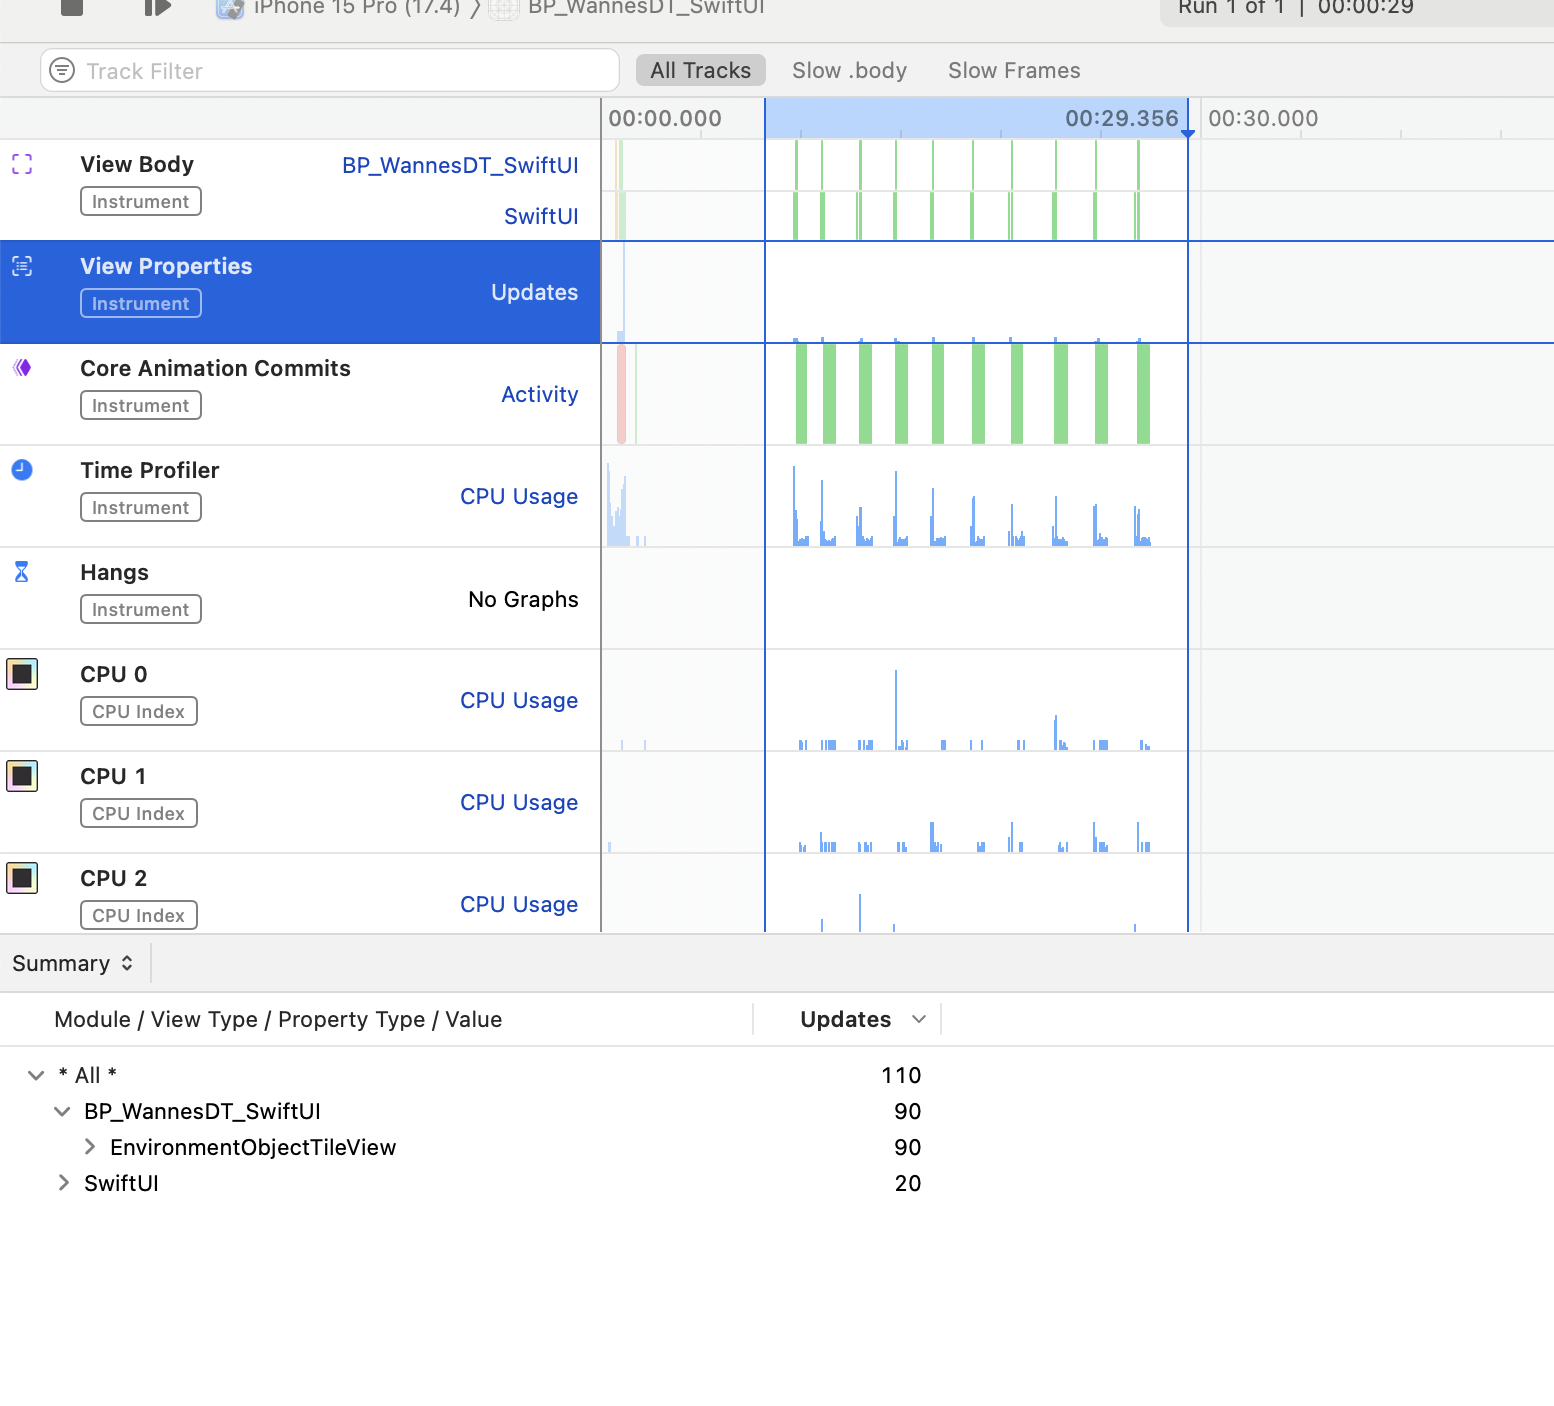
\includegraphics[width=0.7\textwidth]{BPtest2_lazy/EnvironmentObjectPropertyUpdates} 
    \caption{test3: Aantal keren dat de property's updaten bij het meervoudig toewijzigen van een EnvironmentObject}
    \label{fig:propertyUpdatesEnvironmentObject2}
\end{figure}
\paragraph{Totale tijd gebruikt van de CPU}
\begin{figure}[H]
    \centering
    \includegraphics[width=0.7\textwidth]{BPtest2_lazy/EnvironmentObjectTotalCpuTime} 
    \caption{test3: De totale duratie die gebruikt is van de CPU bij het gebruik van EnvironmentObject's}
    \label{fig:cpuUsageTimeEnvironmentObject2}
\end{figure}
\paragraph{Last op de CPU}
\begin{figure}[H]
    \centering
    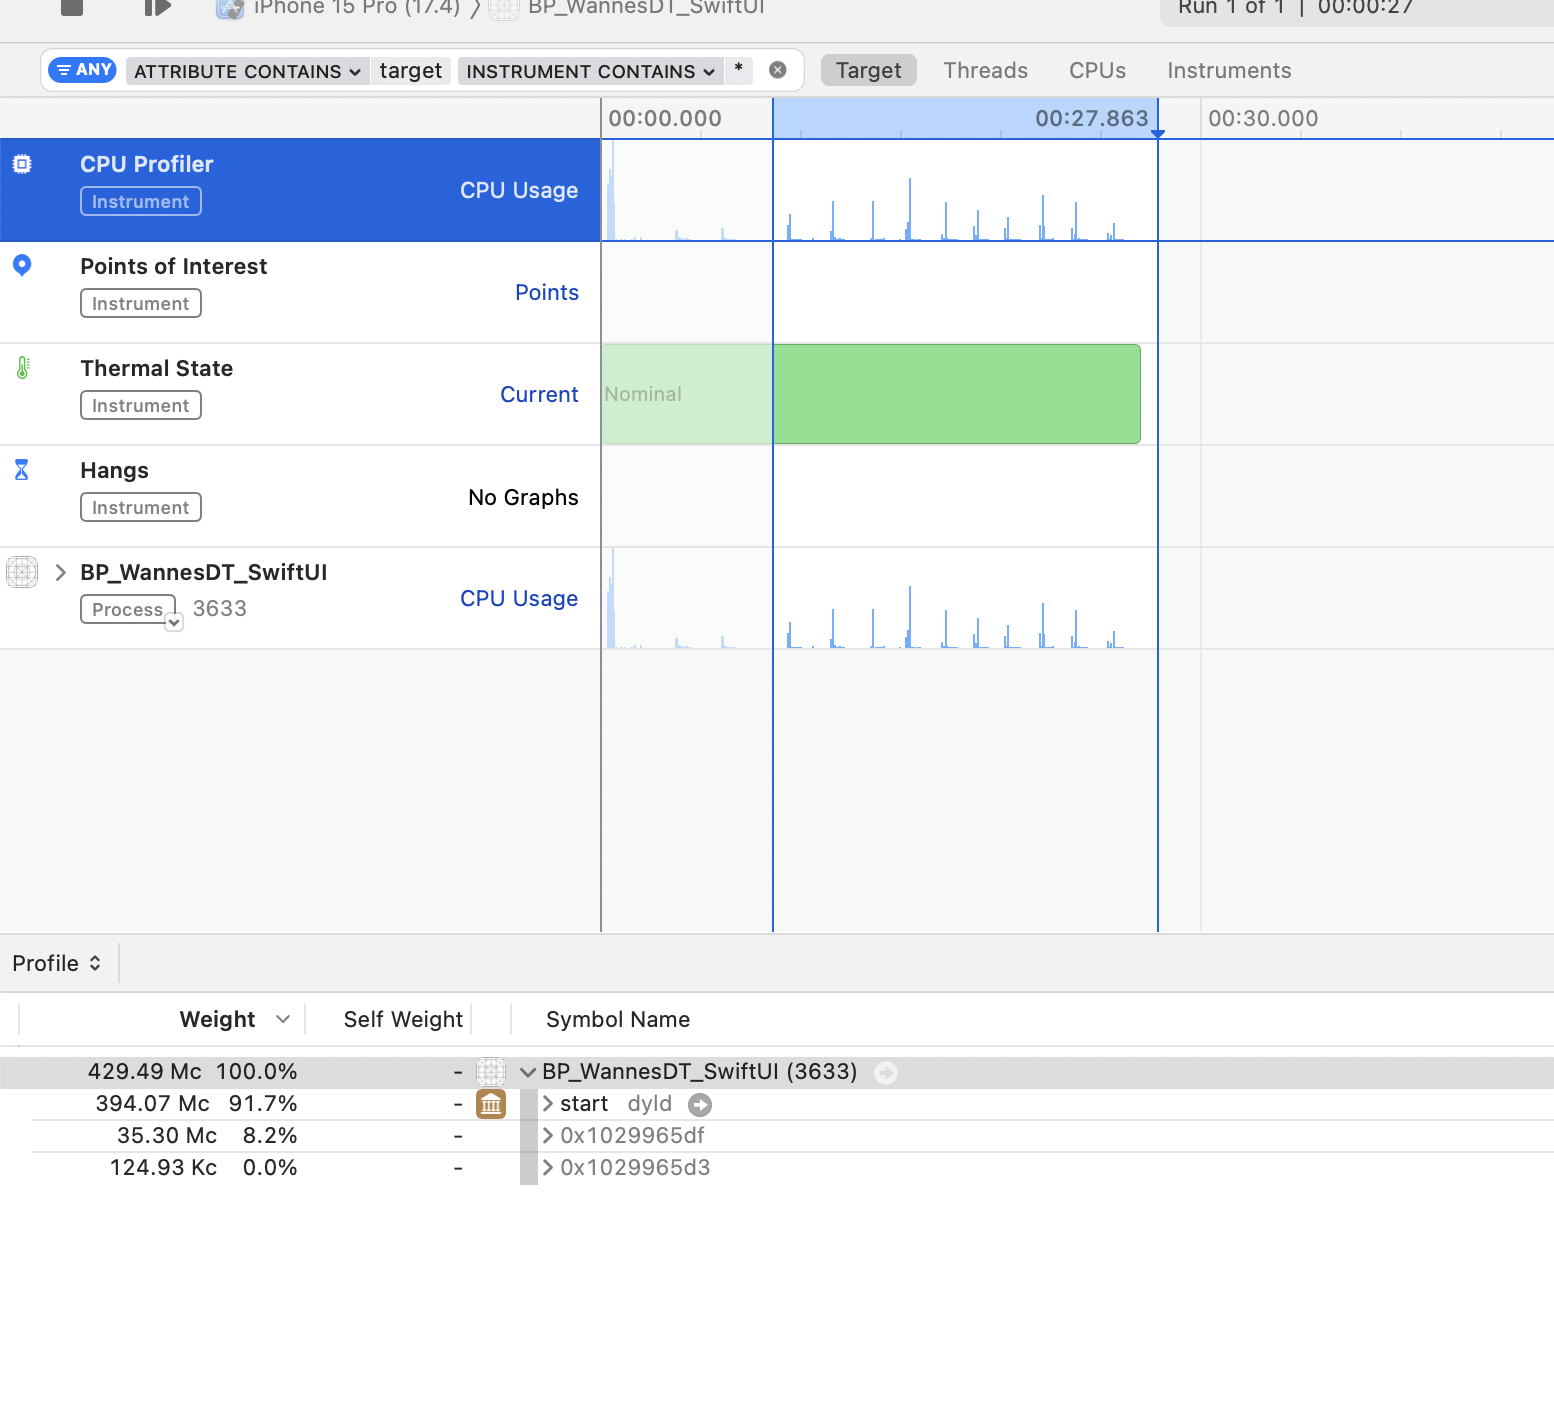
\includegraphics[width=0.7\textwidth]{BPtest2_lazy/EnvironmentObjectCpuWieght} 
    \caption{test3: De totale last van het opnieuw toewijzen van property's op de cpu bij het gebruik van EnvironmentObject's}
    \label{fig:cpuWeightEnvironmentObject2}
\end{figure}

\section{Test4: Dataoverdracht naar meerdere subview's}
\subsection{Binding}
\paragraph{View ververs aantal en ververs tijd}
\begin{figure}[H]
    \centering
    \includegraphics[width=0.7\textwidth]{BPtest2_notlazy/BindingViewRefreshes} 
    \caption{test4: Aantal keren dat de view refreshed en gemiddelde duratie bij het meervoudig toewijzigen van een binding}
    \label{fig:viewRefreshesBinding3}
\end{figure}
\paragraph{Aantal updates van property's}
\begin{figure}[H]
    \centering
    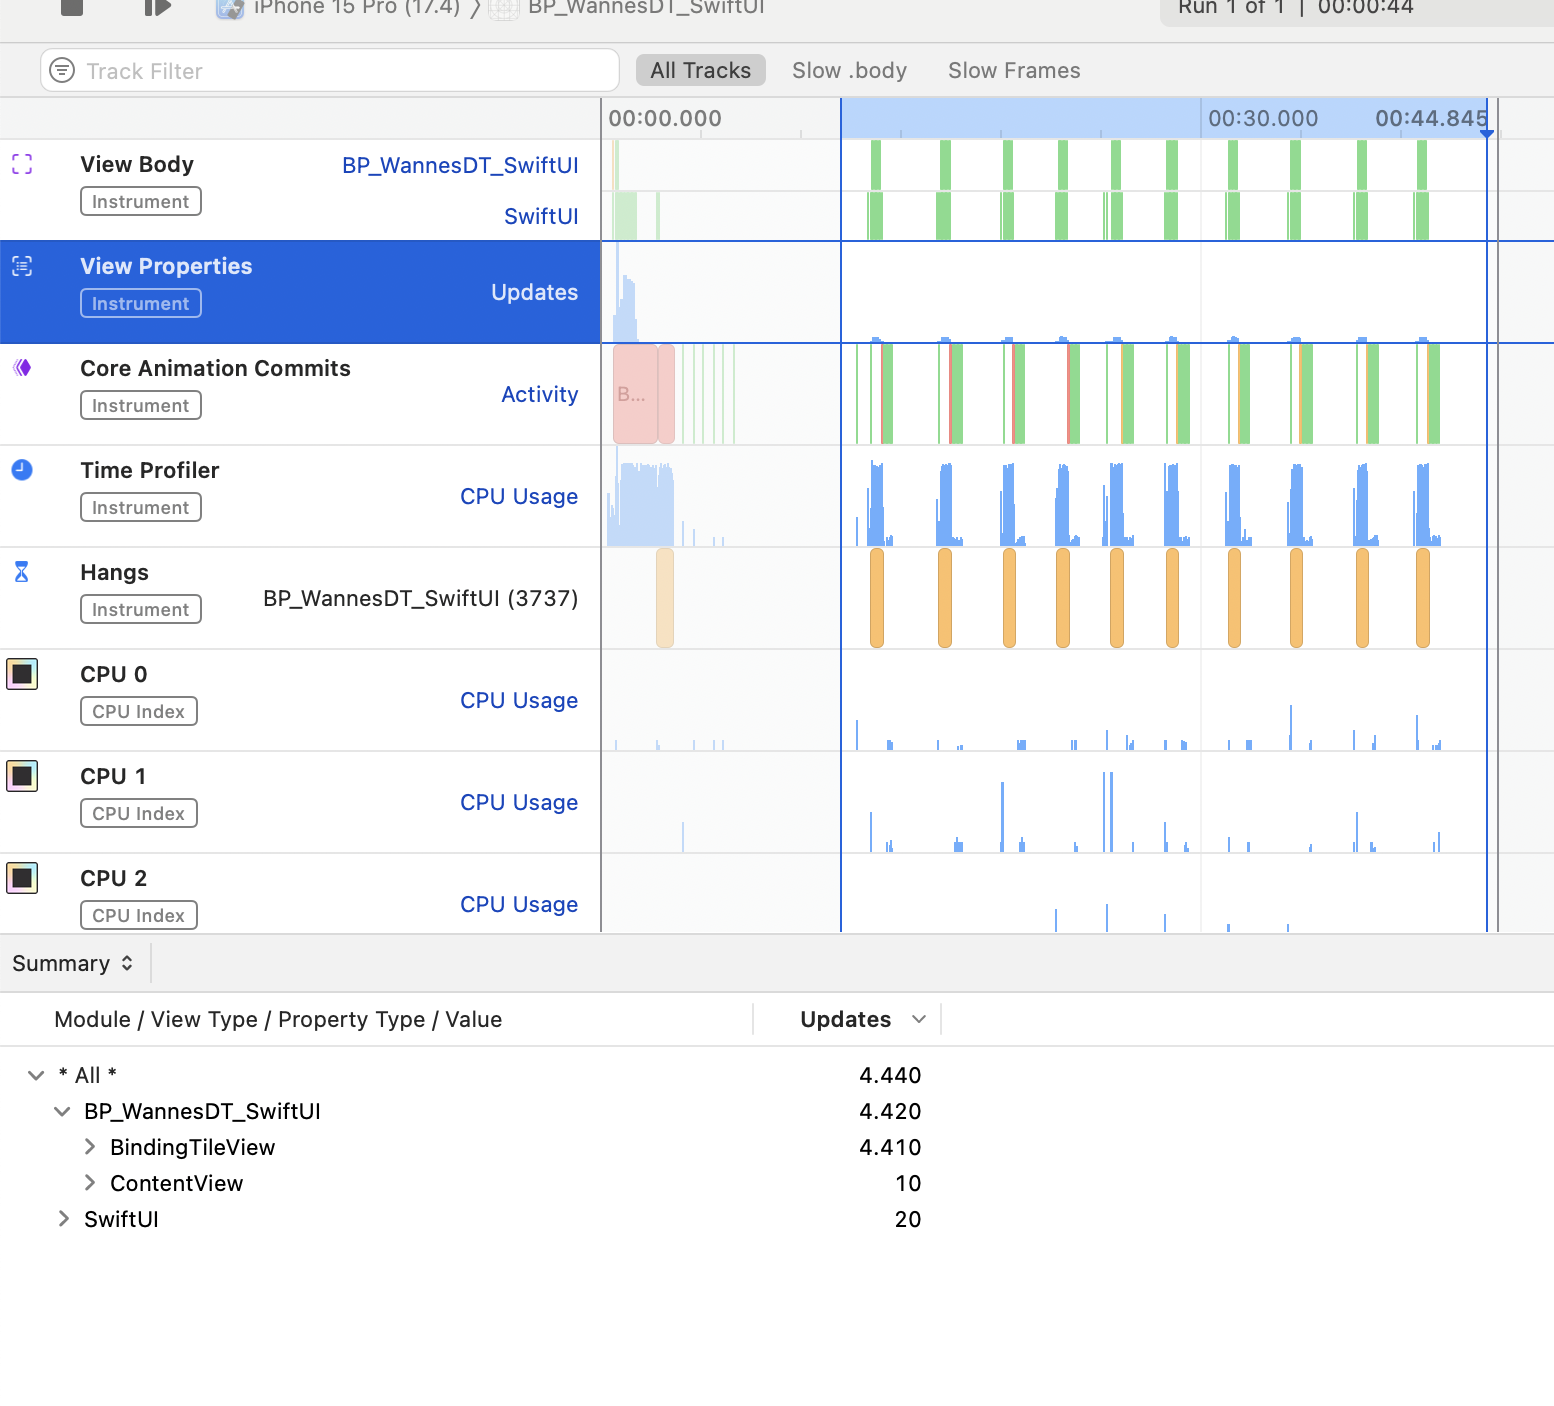
\includegraphics[width=0.7\textwidth]{BPtest2_notlazy/BindingViewPropertyUpdates} 
    \caption{test4: Aantal keren dat de property's updaten bij het meervoudig toewijzigen van een binding}
    \label{fig:propertyUpdatesBinding3}
\end{figure}
\paragraph{Totale tijd gebruikt van de CPU}
\begin{figure}[H]
    \centering
    \includegraphics[width=0.7\textwidth]{BPtest2_notlazy/BindingTotalCpuTime} 
    \caption{test4: De totale duratie die gebruikt is van de CPU bij het gebruik van bindings}
    \label{fig:cpuUsageTimeBinding3}
\end{figure}
\paragraph{Last op de CPU}
\begin{figure}[H]
    \centering
    \includegraphics[width=0.7\textwidth]{BPtest2_notlazy/BindingCpuWeight} 
    \caption{test4: De totale last van het opnieuw toewijzen van property's op de cpu bij het gebruik van bindings}
    \label{fig:cpuWeightBinding3}
\end{figure}

% Observable test 3
\subsection{Observable}
\paragraph{View ververs aantal en ververs tijd}
\begin{figure}[H]
    \centering
    \includegraphics[width=0.7\textwidth]{BPtest2_notlazy/ObservableViewRefreshes} 
    \caption{test4: Aantal keren dat de view refreshed en gemiddelde duratie bij het meervoudig toewijzigen van een Observable}
    \label{fig:viewRefreshesObservable3}
\end{figure}
\paragraph{Aantal updates van property's}
\begin{figure}[H]
    \centering
    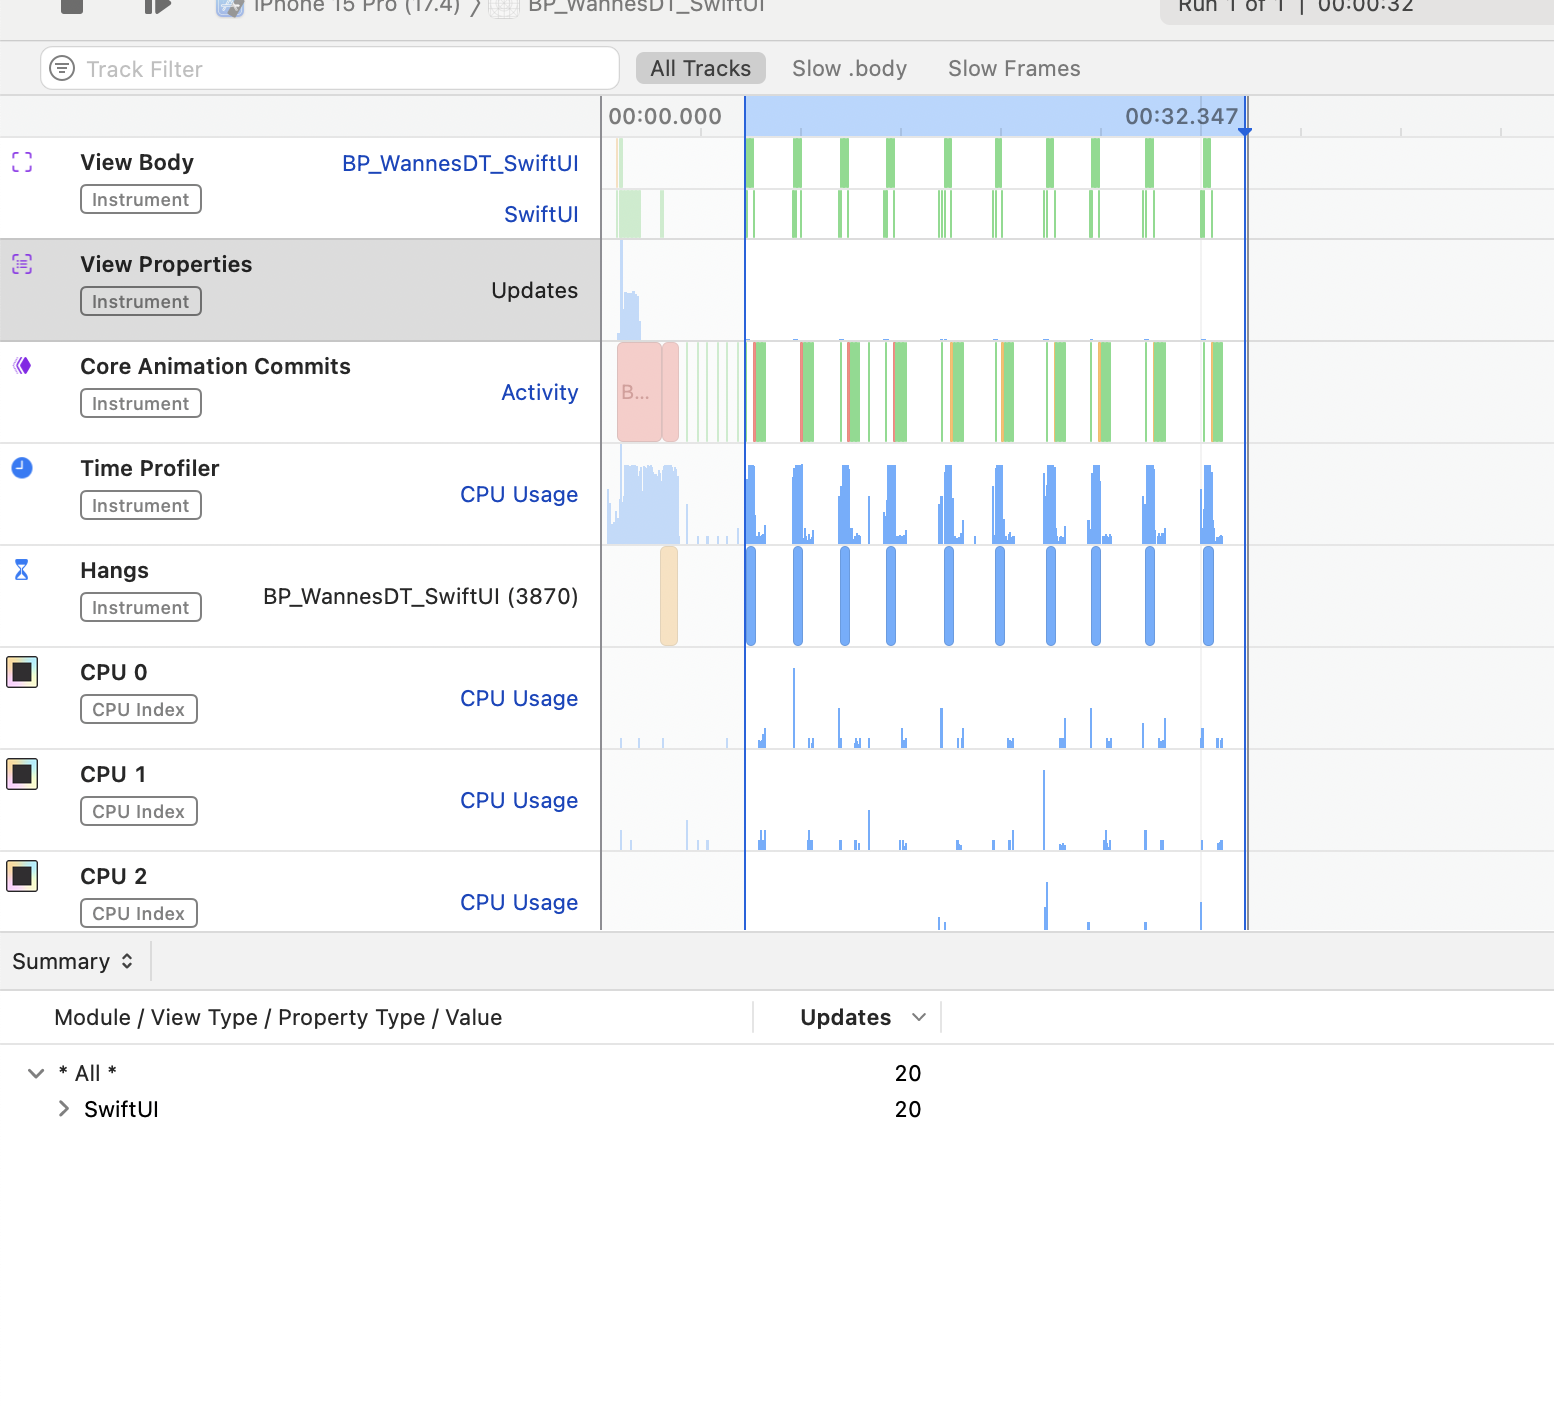
\includegraphics[width=0.7\textwidth]{BPtest2_notlazy/ObservableViewPropertyUpdates} 
    \caption{test4: Aantal keren dat de property's updaten bij het meervoudig toewijzigen van een Observable}
    \label{fig:propertyUpdatesObservable3}
\end{figure}
\paragraph{Totale tijd gebruikt van de CPU}
\begin{figure}[H]
    \centering
    \includegraphics[width=0.7\textwidth]{BPtest2_notlazy/ObservableTotalCpuTime} 
    \caption{test4: De totale duratie die gebruikt is van de CPU bij het gebruik van Observable's}
    \label{fig:cpuUsageTimeObservable3}
\end{figure}
\paragraph{Last op de CPU}
\begin{figure}[H]
    \centering
    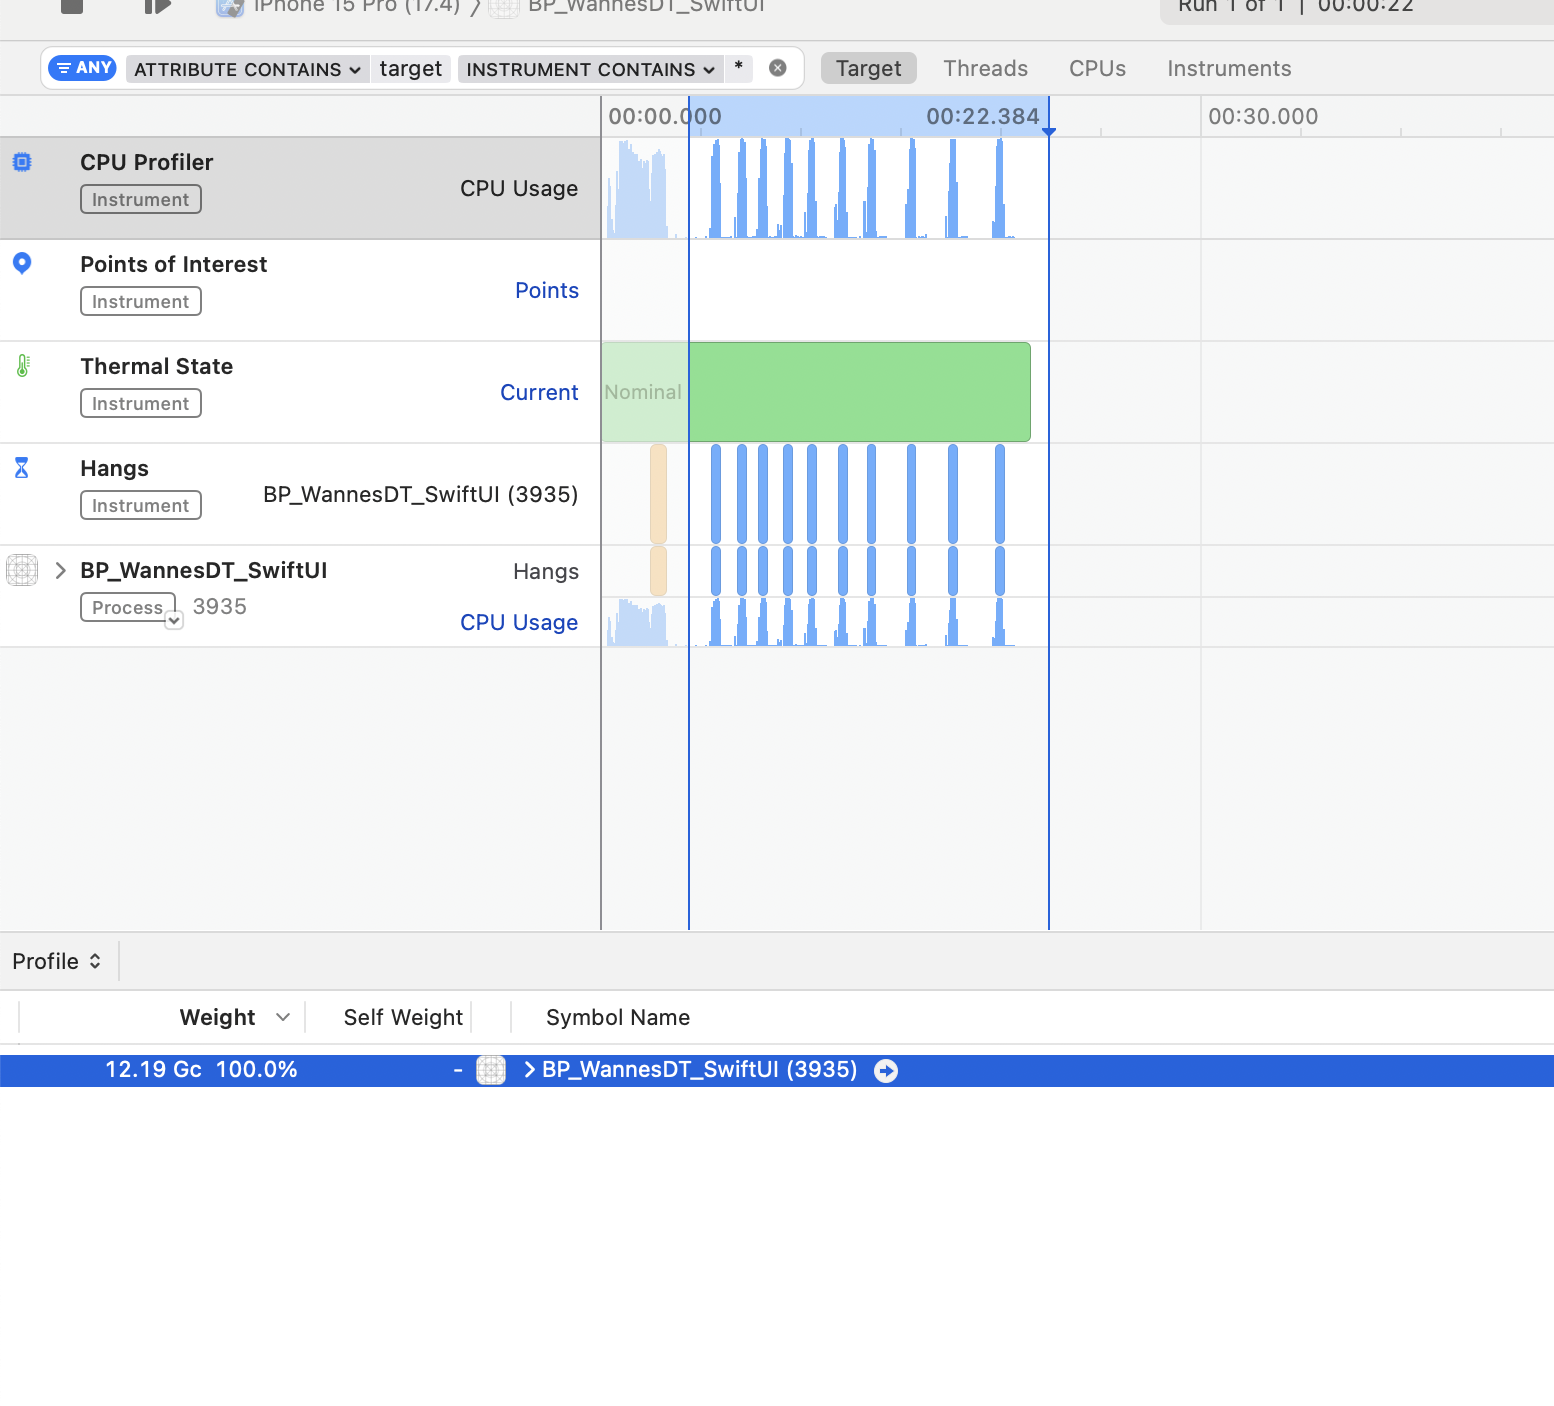
\includegraphics[width=0.7\textwidth]{BPtest2_notlazy/ObservableCpuWeight} 
    \caption{test4: De totale last van het opnieuw toewijzen van property's op de cpu bij het gebruik van Observable's}
    \label{fig:cpuWeightObservable3}
\end{figure}

% ObservedObject test 3
\subsection{ObservedObject}
\paragraph{View ververs aantal en ververs tijd}
\begin{figure}[H]
    \centering
    \includegraphics[width=0.7\textwidth]{BPtest2_notlazy/ObservedObjectViewRefreshes} 
    \caption{test4: Aantal keren dat de view refreshed en gemiddelde duratie bij het meervoudig toewijzigen van een ObservedObject}
    \label{fig:viewRefreshesObservedObject3}
\end{figure}
\paragraph{Aantal updates van property's}
\begin{figure}[H]
    \centering
    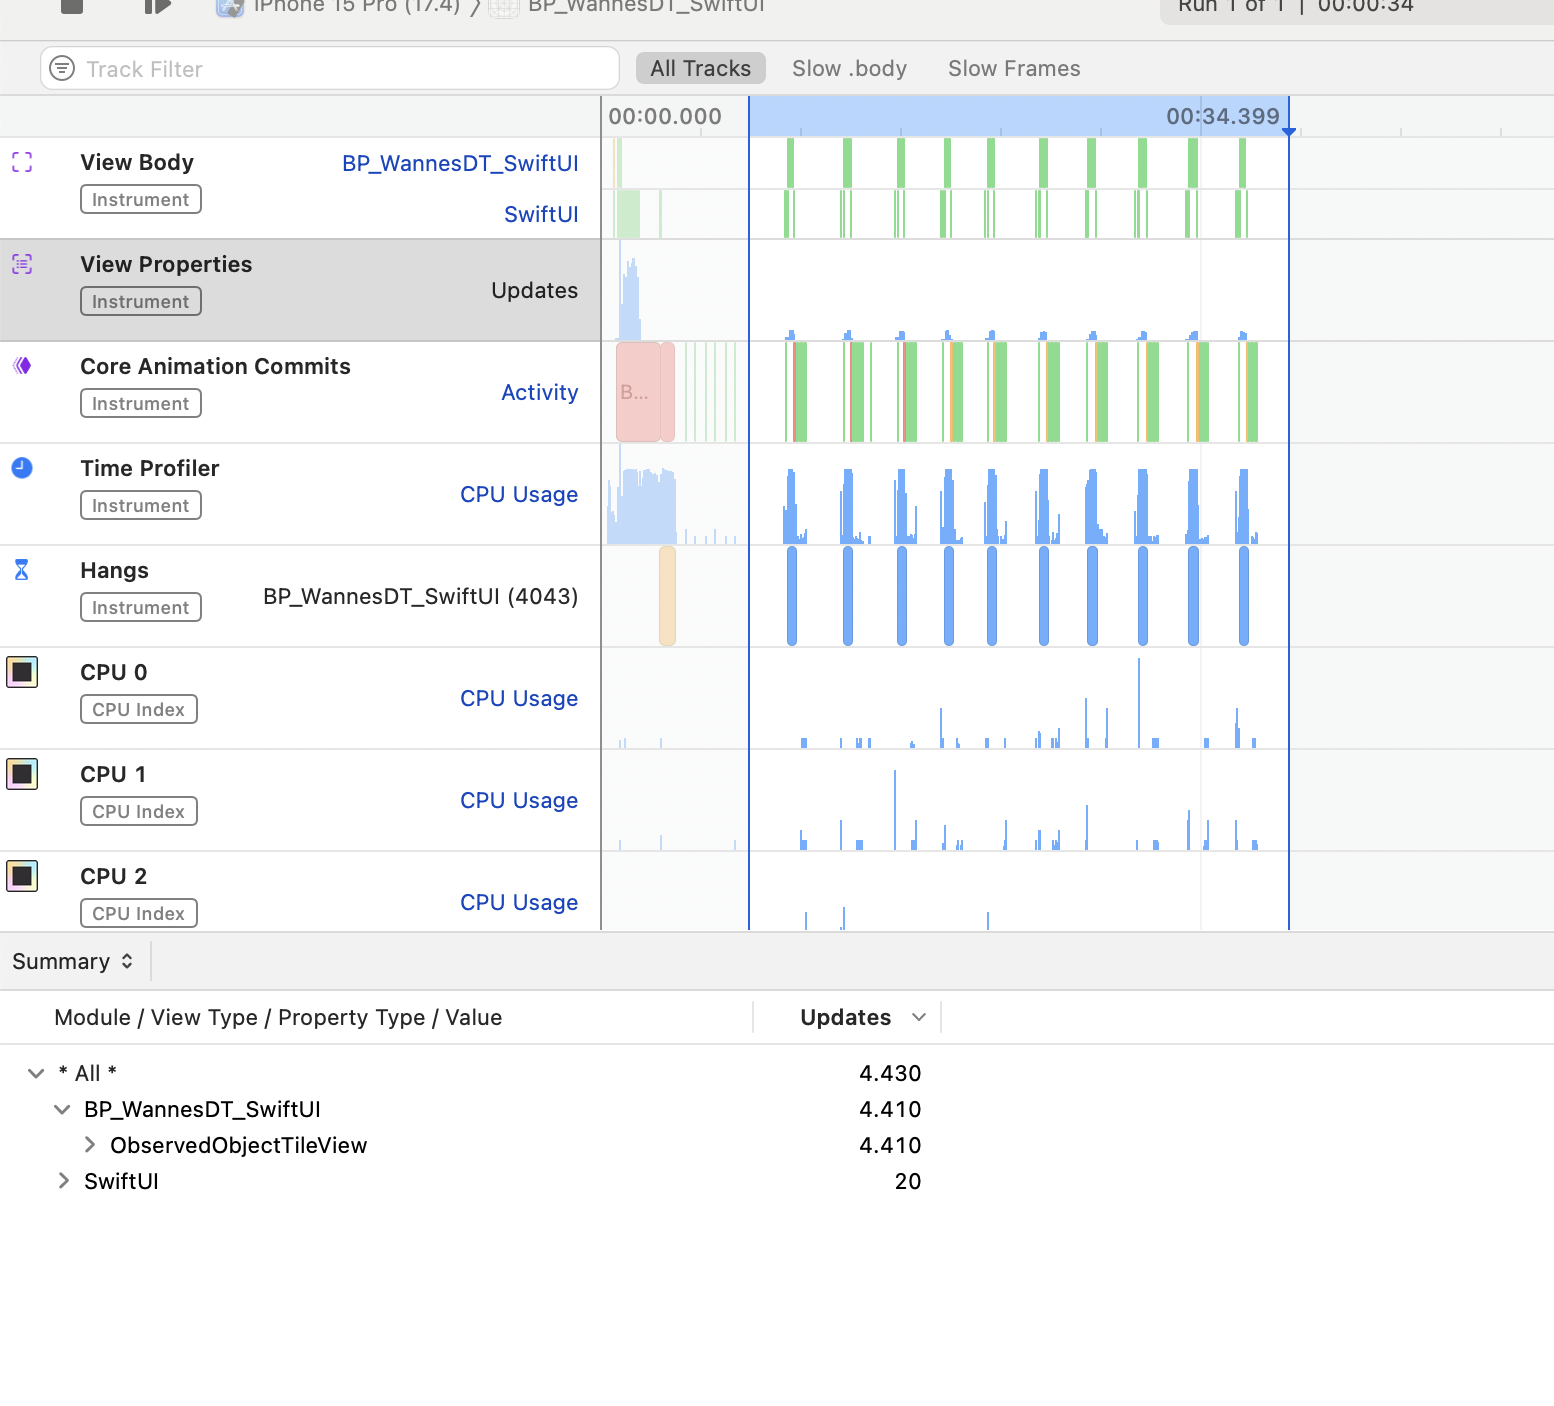
\includegraphics[width=0.7\textwidth]{BPtest2_notlazy/ObservedObjectViewPropertyUpdates} 
    \caption{test4: Aantal keren dat de property's updaten bij het meervoudig toewijzigen van een ObservedObject}
    \label{fig:propertyUpdatesObservedObject3}
\end{figure}
\paragraph{Totale tijd gebruikt van de CPU}
\begin{figure}[H]
    \centering
    \includegraphics[width=0.7\textwidth]{BPtest2_notlazy/ObservedObjectTotalCpuTime} 
    \caption{test4: De totale duratie die gebruikt is van de CPU bij het gebruik van ObservedObject's}
    \label{fig:cpuUsageTimeObservedObject3}
\end{figure}
\paragraph{Last op de CPU}
\begin{figure}[H]
    \centering
    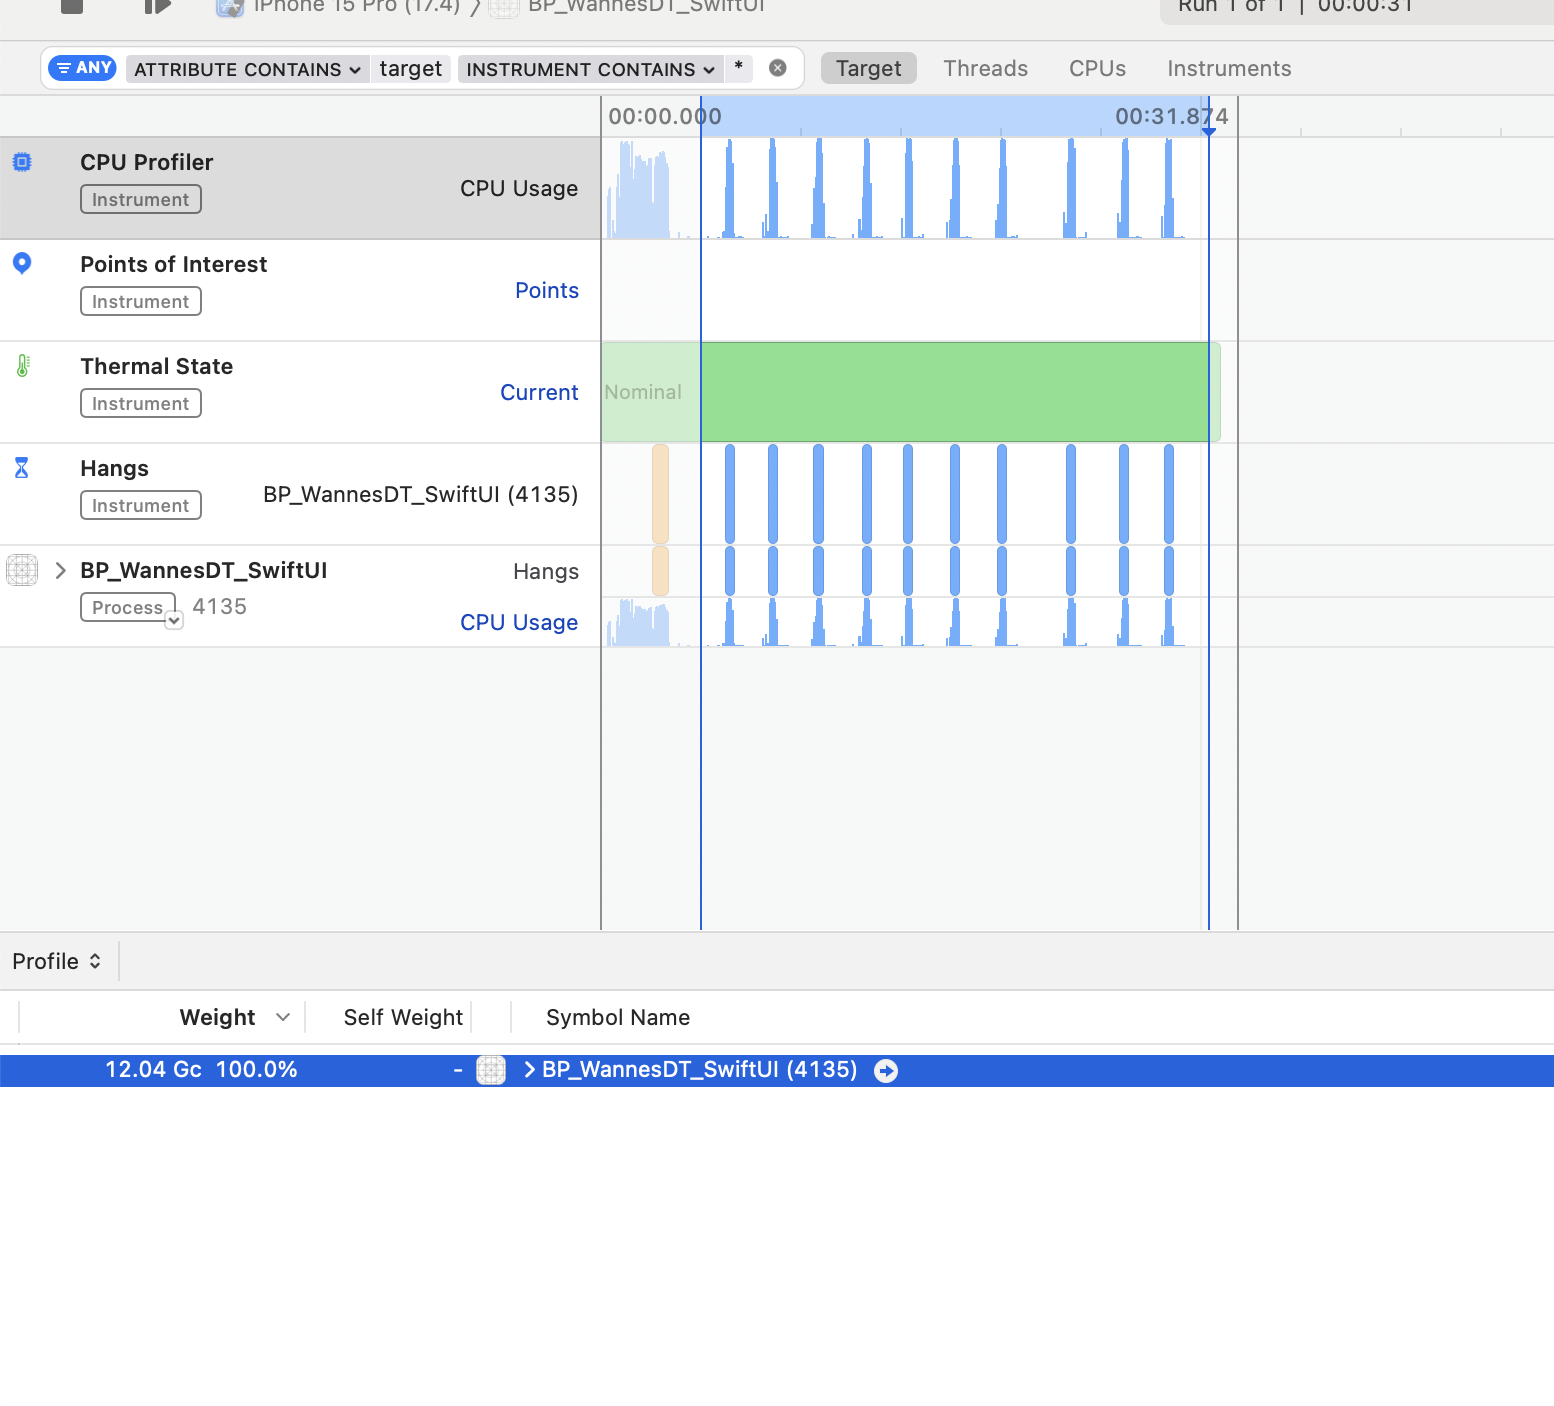
\includegraphics[width=0.7\textwidth]{BPtest2_notlazy/ObservedObjectCpuWeight} 
    \caption{test4: De totale last van het opnieuw toewijzen van property's op de cpu bij het gebruik van ObservedObject's}
    \label{fig:cpuWeightObservedObject3}
\end{figure}

% EnvironmentObject test 3
\subsection{EnvironmentObject}
\paragraph{View ververs aantal en ververs tijd}
\begin{figure}[H]
    \centering
    \includegraphics[width=0.7\textwidth]{BPtest2_notlazy/EnvironmentObjectViewRefreshes} 
    \caption{test4: Aantal keren dat de view refreshed en gemiddelde duratie bij het meervoudig toewijzigen van een EnvironmentObject}
    \label{fig:viewRefreshesEnvironmentObject3}
\end{figure}
\paragraph{Aantal updates van property's}
\begin{figure}[H]
    \centering
    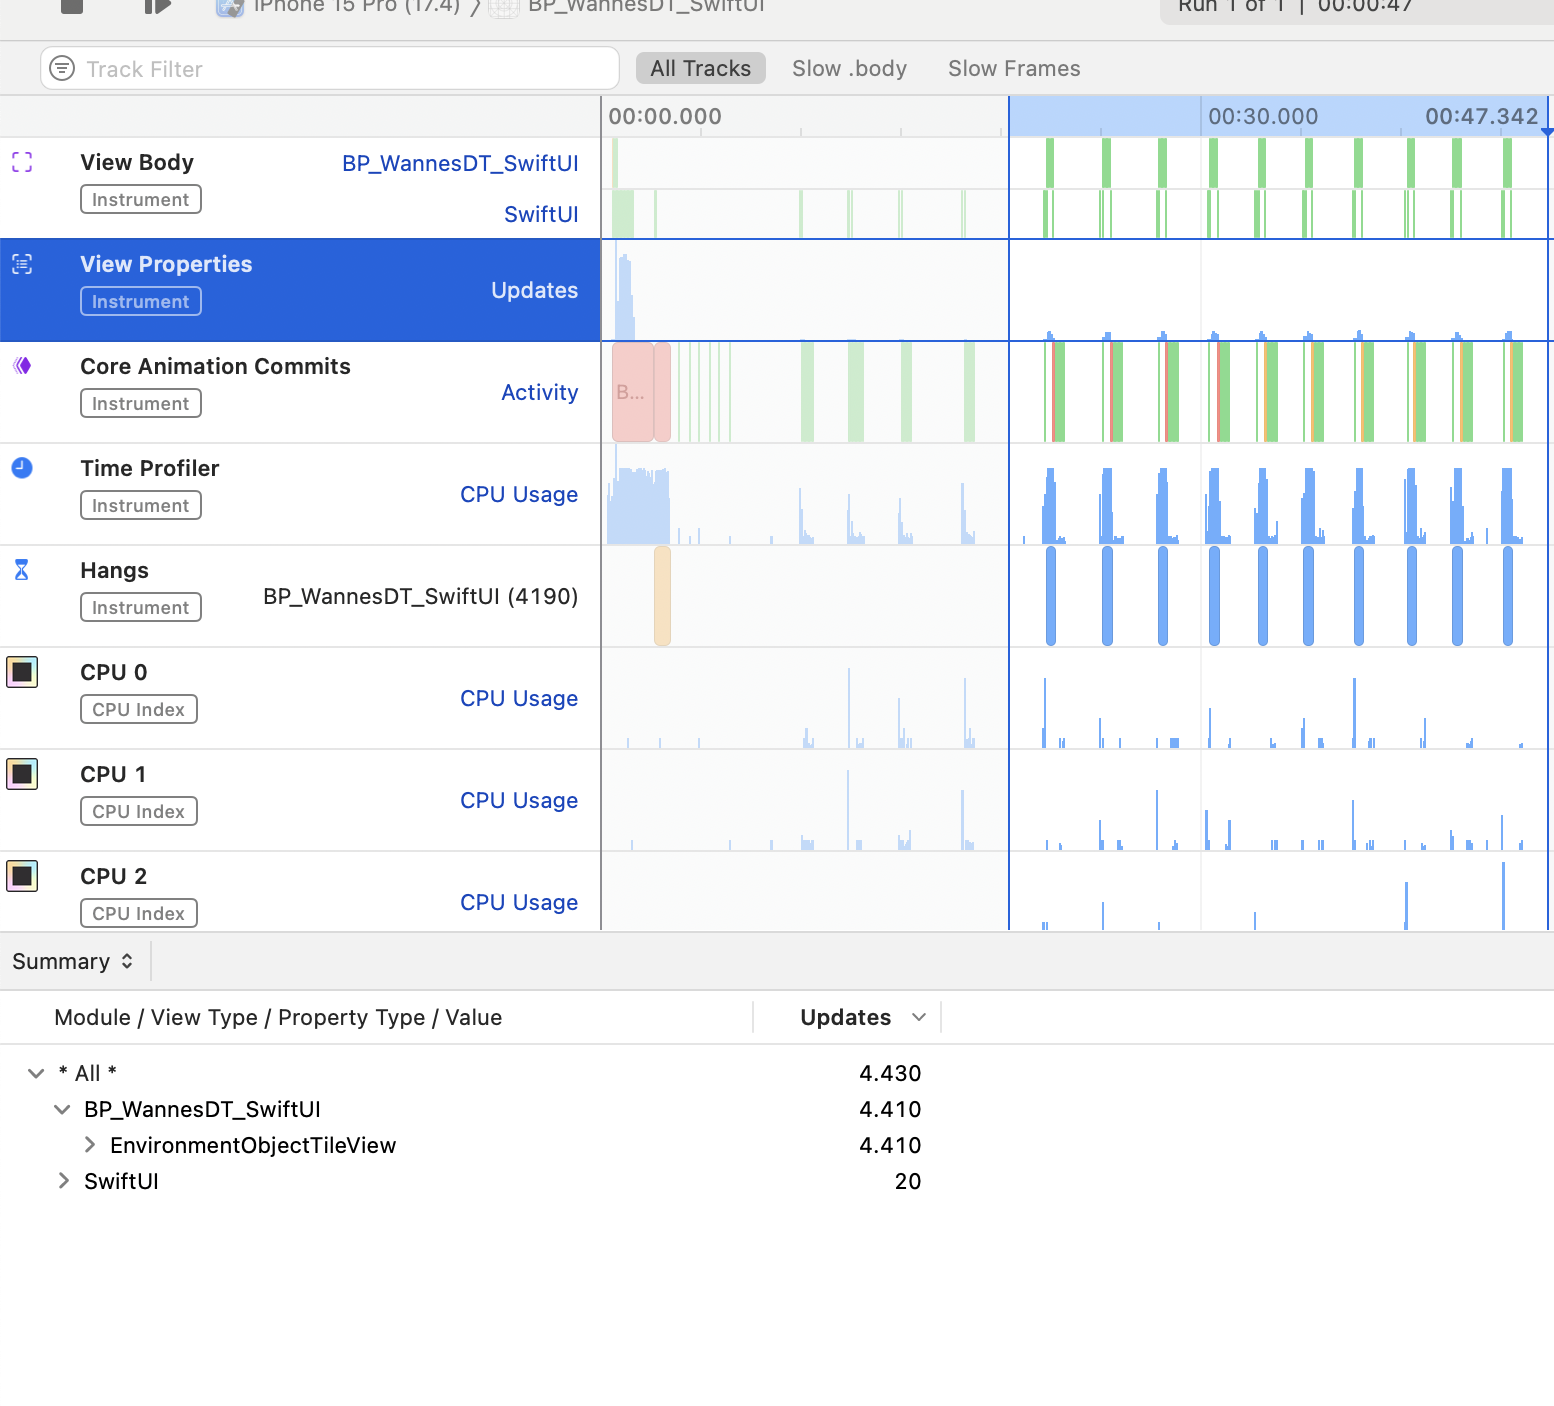
\includegraphics[width=0.7\textwidth]{BPtest2_notlazy/EnvironmentObjectViewPropertyUpdates} 
    \caption{test4: Aantal keren dat de property's updaten bij het meervoudig toewijzigen van een EnvironmentObject}
    \label{fig:propertyUpdatesEnvironmentObject3}
\end{figure}
\paragraph{Totale tijd gebruikt van de CPU}
\begin{figure}[H]
    \centering
    \includegraphics[width=0.7\textwidth]{BPtest2_notlazy/EnvironmentObjectTotalCpuTime} 
    \caption{test4: De totale duratie die gebruikt is van de CPU bij het gebruik van EnvironmentObject's}
    \label{fig:cpuUsageTimeEnvironmentObject3}
\end{figure}
\paragraph{Last op de CPU}
\begin{figure}[H]
    \centering
    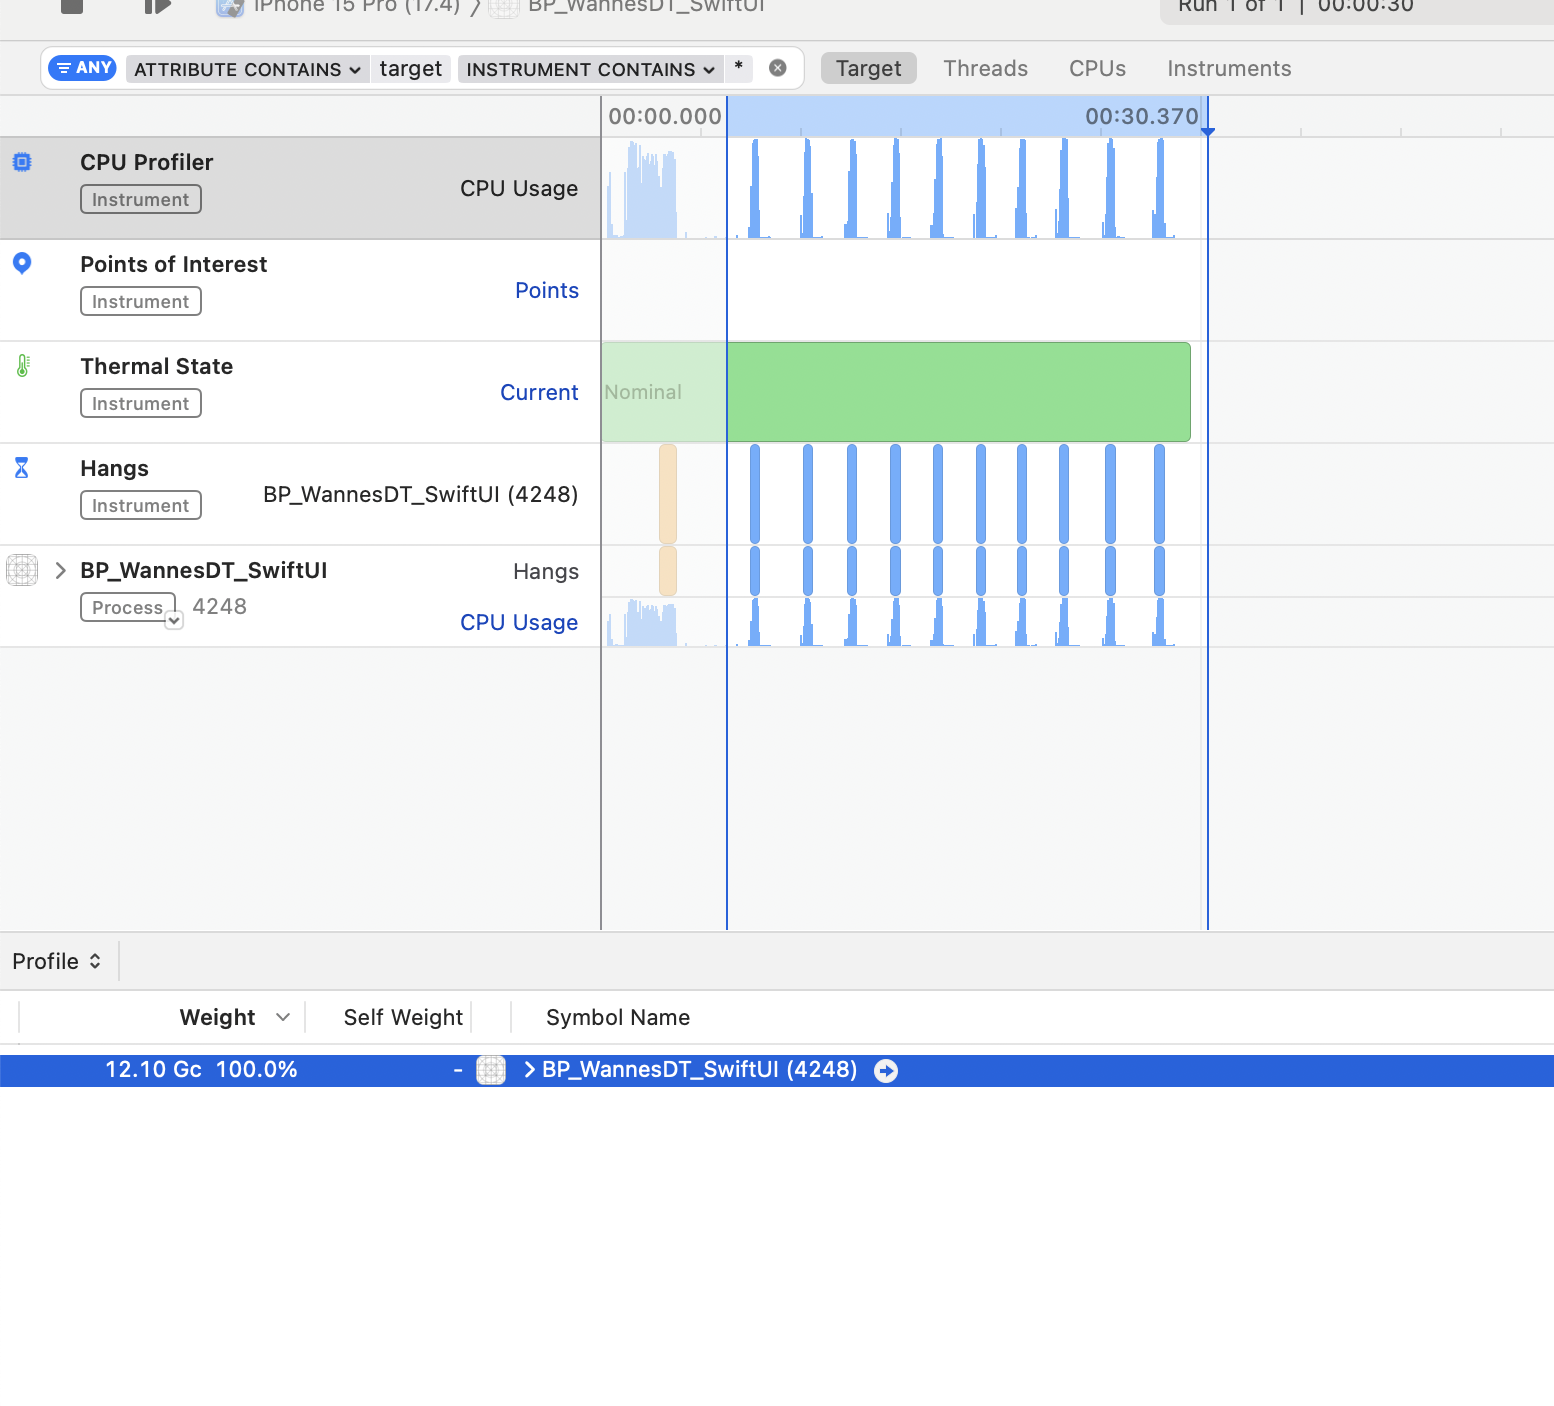
\includegraphics[width=0.7\textwidth]{BPtest2_notlazy/EnvironmentObjectCpuWeight} 
    \caption{test4: De totale last van het opnieuw toewijzen van property's op de cpu bij het gebruik van EnvironmentObject's}
    \label{fig:cpuWeightEnvironmentObject3}
\end{figure}